\documentclass[12pt]{article}
\usepackage{makecell}
\usepackage{hyphenat}
\usepackage[utf8]{vietnam}
\usepackage[vietnamese=nohyphenation]{hyphsubst}
\usepackage[vietnamese]{babel}
\usepackage[table,dvipsnames]{xcolor} % Required for row coloring
\usepackage{booktabs} % Required for nicer horizontal lines
\usepackage{ragged2e}
\usepackage{caption}
\usepackage{subcaption}
\usepackage{float}
\usepackage{amsmath,amssymb,amsfonts}
\usepackage{graphicx}
\usepackage{adjustbox}
\usepackage{multicol}
\usepackage[inline,shortlabels]{enumitem}
\usepackage{setspace}
\usepackage{longtable}
\usepackage{bm} 
\usepackage[inkscapelatex=false]{svg}
\usepackage{titling}
\usepackage{tabularx}
\usepackage[T1]{fontenc}
\usepackage{lmodern,mathrsfs}
% \usepackage[draft]{hyperref}
\usepackage{hyperref}
\usepackage{xparse}
\usepackage{fontawesome5}
\usepackage[most]{tcolorbox}
\usepackage{tikz}
\usepackage[framemethod=TikZ]{mdframed}
\usetikzlibrary{matrix, fit, shadows, positioning, arrows.meta, calc, shapes.geometric, backgrounds, shapes.symbols}
\usepackage{paracol}
\usepackage{bbm}
\usepackage{pgfplots}
\usepackage{siunitx}
\usepackage{multirow}
%  biblatex (thay cho IEEEtran.bst) ------------------------------------
\usepackage[
    backend=bibtex,
    style=ieee,
    citestyle=numeric-comp,
    maxnames=1,     % chỉ hiển thị 1 tên tác giả, phần còn lại thành ``et al."
    minnames=1,
    uniquelist=false,
    hyperref=false
]{biblatex}
\usepackage{forest}
\addbibresource{references.bib}
\DefineBibliographyStrings{english}{
  andothers = {et\addabbrvspace al\adddot}
}
\AtBeginBibliography{\selectlanguage{english}}

% -----------------------------------------------------------------
\AtBeginDocument{\renewcommand\refname{}}

\usepackage[toc,page]{appendix}
\renewcommand{\appendixtocname}{Phụ lục}      
\renewcommand{\appendixpagename}{Phụ lục}

\usepackage{xurl}
\setlength{\headheight}{14.5pt}
\setlength{\topmargin}{-.5in} \setlength{\textheight}{9.25in}
\setlength{\oddsidemargin}{-0.1in} \setlength{\textwidth}{6.8in}

\usepackage{tocloft}
\renewcommand{\cfttoctitlefont}{\Huge\bfseries}
\setlength{\cftaftertoctitleskip}{2em}
\setlength{\cftbeforesubsecskip}{7pt} % giãn cách subitem mục lục
\renewcommand{\cftsecleader}{\cftdotfill{\cftdotsep}}
\setlength{\cftsecnumwidth}{3em}
\renewcommand{\cftsecaftersnum}{\quad}
\renewcommand{\cftsubsecleader}{\cftdotfill{\cftdotsep}}
\setlength{\cftsubsecnumwidth}{4em}
\renewcommand{\cftsubsecaftersnum}{\quad}
\renewcommand{\cftsubsubsecleader}{\cftdotfill{\cftdotsep}}
\setlength   {\cftsubsubsecnumwidth}{5em}  
\renewcommand{\cftsubsubsecaftersnum}{\quad}

\PassOptionsToPackage{vietnamese.licr}{babel}
\usepackage{vipythonhighlight}
\usepackage{tvietlistings}


%--------------------------------------------------------------------
\usepackage{framed}
\usepackage{fancyhdr}
\usepackage{upquote}
\usepackage{listings}	 
	    

% Color --------------------------------------------------------------------
\usepackage{epigraph}
\usepackage{titlesec}

\definecolor{codebackground}{RGB}{250, 250, 250}
\definecolor{codecomment}{RGB}{34, 139, 34}
\definecolor{codekeyword}{RGB}{0, 0, 255}
\definecolor{codestring}{RGB}{255, 0, 0}
\definecolor{codeidentifier}{RGB}{0, 0, 0}
\definecolor{codelinenumbers}{RGB}{90, 90, 90}

\definecolor{codegreen}{rgb}{0,0.6,0}
\definecolor{codegray}{rgb}{0.5,0.5,0.5}
\definecolor{codepurple}{rgb}{0.58,0,0.82}
\definecolor{backcolour}{rgb}{0.95,0.95,0.92}

\definecolor{aivnGreen}{RGB}{52,79,30}  
\definecolor{aivnCodeOutputColor}{RGB}{11,83,148}  
\definecolor{captiongray}{gray}{0.15} 
\definecolor{captionbg}{RGB}{250,250,250}

\definecolor{foldercolor}{RGB}{0, 102, 204}
\definecolor{filecolor}{RGB}{104, 104, 104}
\definecolor{scriptcolor}{RGB}{180, 50, 50}
\definecolor{pythoncolor}{RGB}{0, 128, 128}

% --- Extra Brand colors for the table ---
\definecolor{brandIndigo}{HTML}{333D91} 
\definecolor{rowLavender}{HTML}{EEECFA}
\setlength{\parskip}{0.3em}

% Table
\newtcolorbox{captionbelowboxaivn}{
    colback=aivnGreen,
    colframe=aivnGreen,
    boxrule=0pt,
    arc=4pt,
    left=4pt,
    right=4pt,
    top=2pt,
    bottom=2pt,
    width=\linewidth,
    boxsep=4pt,
    halign=center,
    % fontupper=\bfseries\color{white}
    fontupper=\color{white}
}

% Figure
\newtcolorbox{figurecardcaptionaivn}{
  colback=aivnGreen,        % Màu nền (background color)
  colframe=aivnGreen,       % Màu viền box (border color)
  boxrule=0pt,              % Độ dày viền box (0pt = không viền)
  arc=2pt,                  % Độ bo góc (2pt là bo nhẹ, tăng để bo tròn hơn)
  top=3pt,                  % Padding phía trên nội dung
  bottom=3pt,               % Padding phía dưới nội dung
  left=10pt,                % Padding bên trái
  right=10pt,               % Padding bên phải
  width=\linewidth,         % Chiều rộng bằng toàn bộ dòng
  fontupper=\small\fontsize{11pt}{13pt}\selectfont\color{white} 
}

% Tạo counter riêng
\newcounter{hinh}
% Định nghĩa macro caption Hình
\newcommand{\capfig}[1]{%
  \refstepcounter{hinh}%
  % \textbf{Hình~\thehinh:}~#1
    Hình~\thehinh:~#1
}

\newtcolorbox{figurecaptionmodern}{
  colback=captionbg,
  colframe=aivnGreen,
  boxrule=1.5pt,
  bottomrule=2pt,  
  toptitle=0pt,
  bottomtitle=0pt,
  left=6pt,
  right=6pt,
  top=4pt,
  bottom=2pt,
  width=\linewidth,
  fontupper=\small\fontsize{11pt}{13pt}\selectfont\color{black},
  halign=center
}

% Code Block -----------------------------------------------------------------
\newtcolorbox{aivncodebox}[1][]{%
  enhanced,
  colback=gray!10,
  colframe=aivnGreen,
  coltitle=white,
  colbacktitle=aivnGreen,
  title=#1,
  fonttitle=\bfseries\sffamily,
  listing only,
  breakable,
  listing engine=listings,
  listing options={
    language=Python,
    basicstyle=\ttfamily\footnotesize,
    commentstyle=\color{ForestGreen},
    keywordstyle=\color{blue},
    stringstyle=\color{red!70!black},
    numbers=left, upquote=true,
    numberstyle=\tiny\color{gray},
    numbersep=5pt,
    breaklines=true,
    showstringspaces=false,
    xleftmargin=1.5em,
    framexleftmargin=1.5em
  }
}

% Code Output Block -----------------------------------------------------------------
\newtcolorbox{aivnCodeOutput}[1][]{%
  enhanced,
  colback=gray!10,
  colframe=aivnCodeOutputColor,
  coltitle=white,
  colbacktitle=aivnCodeOutputColor,
  title=#1,
  fonttitle=\bfseries\sffamily,
  listing only,
  breakable,
  listing engine=listings,
  listing options={
    language=Python,
    basicstyle=\ttfamily\footnotesize,
    commentstyle=\color{ForestGreen},
    keywordstyle=\color{blue},
    stringstyle=\color{red!70!black},
    numbers=left,
    numberstyle=\tiny\color{gray},
    numbersep=5pt,
    breaklines=true,
    showstringspaces=false,
    xleftmargin=1.5em,
    framexleftmargin=1.5em
  }
}

% Last argument allows more tcolorbox options to be added

% --- Guideline/Tip box ---
\newtcolorbox{guidelinebox}[2][]{
    enhanced, colback=yellow!10!white, colframe=orange!90!black, boxrule=1pt, arc=4pt,
    fonttitle=\bfseries, attach boxed title to top left={yshift=-2mm, xshift=3mm},
    colbacktitle=orange!90!black, coltitle=white,
    title=\faLightbulb\hspace{1mm} #2, #1
}

\newtcolorbox{notebox}[1][]{
  enhanced,  colback=yellow!10, colframe=orange!80, boxrule=1pt, 
  arc=4pt, fontupper=\small, attach boxed title to top left={yshift=-2mm, xshift=3mm},
  colbacktitle=orange!80,  coltitle=white, fonttitle=\bfseries,  
  title=\faInfoCircle~\textbf{Lưu ý},  #1
}

\newtcolorbox{infobox}[1]{%
    enhanced, 
    breakable, 
    colback=green!3, 
    colframe=green!3, 
    arc=5pt,
    borderline west={3pt}{0pt}{aivnGreen},
    attach boxed title to top left={ 
        yshift*=-\tcboxedtitleheight/2, 
        xshift=-0.1em 
    },
    colbacktitle=aivnGreen, %
    coltitle=white, 
    fonttitle=\bfseries, 
    boxed title style={ 
        arc=4pt, 
        top=2pt, 
        bottom=2pt,
        left=8pt,
        right=8pt,
    },
    title={\faInfoCircle\quad #1}
}
\newtcolorbox{examplebox}[1]{%
    enhanced,
    breakable,
    colback=brandIndigo!5,      
    colframe=brandIndigo!5,     
    arc=5pt,
    borderline west={3pt}{0pt}{brandIndigo}, 
    attach boxed title to top left={
        yshift*=-\tcboxedtitleheight/2,
        xshift=-0.1em
    },
    colbacktitle=brandIndigo,   
    coltitle=white,
    fonttitle=\bfseries,
    boxed title style={
        arc=4pt,
        top=2pt,
        bottom=2pt,
        left=8pt,
        right=8pt,
    },
    title={\faLightbulb\quad #1} 
}
% Prompt Block ---------------------------------------------------------------
\definecolor{promptBlue}{HTML}{2F5D8C}
\definecolor{promptBg}{HTML}{F6F9FC}
\definecolor{promptBorder}{HTML}{B7C9DC}

% Dùng cho prompt đã viết theo cú pháp LaTeX bình thường
\newtcolorbox{promptbox}[1][Prompt]{%
    enhanced,
    breakable,
    colback=promptBg,
    colframe=promptBorder,
    coltitle=white,
    colbacktitle=promptBlue,
    fonttitle=\bfseries\sffamily,
    title={#1},
    boxrule=0.8pt,
    arc=4pt,
    left=8pt,
    right=8pt,
    top=2pt,
    bottom=1pt,
    before skip=8pt,
    after skip=8pt,
    borderline west={3pt}{0pt}{promptBlue},
    fontupper=\small\sffamily,
}

% Dùng cho prompt raw: giữ nguyên xuống dòng, không highlight keyword
\newtcblisting{promptboxraw}[1][Prompt]{%
    enhanced,
    breakable,
    listing only,
    listing engine=listings,
    colback=promptBg,
    colframe=promptBorder,
    coltitle=white,
    colbacktitle=promptBlue,
    fonttitle=\bfseries\sffamily,
    title={#1},
    boxrule=0.8pt,
    arc=4pt,
    left=8pt,
    right=8pt,
    top=-4pt,
    bottom=-4pt,
    before skip=4pt,
    after skip=4pt,
    borderline west={3pt}{0pt}{promptBlue},
    listing options={
        language={},
        basicstyle=\small\ttfamily,
        columns=fullflexible,
        keepspaces=true,
        breaklines=true,
        showstringspaces=false,
        numbers=none,
        frame=none,
        keywordstyle=\color{black},
        commentstyle=\color{black},
        stringstyle=\color{black},
        identifierstyle=\color{black}
    }
}


%--------------------------------------------------------------------
\lstdefinestyle{mystyle}{
    backgroundcolor=\color{codebackground},
    commentstyle=\color{codecomment},
    keywordstyle=\color{codekeyword},
    stringstyle=\color{codestring},
    identifierstyle=\color{codeidentifier},
    basicstyle=\ttfamily\footnotesize,
    breakatwhitespace=false,
    breaklines=true,
    captionpos=b,
    keepspaces=true,
    numbers=left,
    numberstyle=\tiny\color{codelinenumbers}, 
    numbersep=5pt,
    showspaces=false,
    showstringspaces=false,
    showtabs=false,
    tabsize=2
}

\lstset{style=mystyle}

\hypersetup{
    colorlinks=true,
    linkcolor=black,
    filecolor=magenta,    
    citecolor=green,
    urlcolor=blue,
    pdftitle={Nguyen nhan va co che bien doi gradient trong mang no-ron sau},
    pdfpagemode=FullScreen,
}

%--------------------------------------------------------------------
\newcounter{choice}
\renewcommand\thechoice{($\alph{choice}$)}
\newcommand\choicelabel{\thechoice}

%--------------------------------------------------------------------
\newenvironment{choices}%
  {\list{\choicelabel}%
     {\usecounter{choice}\def\makelabel##1{\hss\llap{##1}}%
       \settowidth{\leftmargin}{W.\hskip\labelsep\hskip 0 em}%
       \def\choice{%
         \item
       } % choice
       \labelwidth\leftmargin\advance\labelwidth-\labelsep
       \topsep=0pt
       \partopsep=0pt
     }%
  }%
  {\endlist}
  
%--------------------------------------------------------------------
\def\CChoice{%
      \choice
      \addanswer{\theenumi}{\thechoice}%
    }
    \let\CChoice\CChoice
%    \par % Uncomment this to have choices always start a new line
   % \let\par\@empty
    % If we're continuing the textbf containing the question,
    % then leave a bit of space before the first choice:
    \ifvmode\else\enskip\fi
    \ignorespaces
  %
  {}
\makeatother
\newbox\allanswers
\setbox\allanswers=\hbox{}
\newcommand{\addanswer}[2]{%
  \global\setbox\allanswers=\hbox{\unhbox\allanswers \quad #1.~#2}%
}
\newcommand{\showanswers}{%
  \vfill
  \begin{center}
    Answers
  \end{center}
  \unhbox\allanswers
}

\makeatletter
\newenvironment{multichoices}[1][1]{%
\begin{multicols}{#1}}{%
\end{multicols}}
\makeatother

\pagestyle{fancy}

\DeclareMathOperator*{\argmax}{arg\,max}
\DeclareMathOperator*{\argmin}{arg\,min}
\DeclareMathOperator{\E}{\mathbb{E}}

% Outline --------------------------------------------------------------------
% Section numbering ----------------------------------------------------------
\renewcommand{\thesection}{\Roman{section}.} 
\renewcommand{\thesubsection}{\thesection\arabic{subsection}.}
\renewcommand{\thesubsubsection}{\thesubsection\arabic{subsubsection}.}

% Paper-like section title sizes --------------------------------------------
% Title paper: 17pt
% Section should be clearly smaller than title but still prominent.
\titleformat{\section}
  {\normalfont\fontsize{16pt}{20pt}\selectfont\bfseries}
  {\thesection}
  {0.85em}
  {}

\titleformat{\subsection}
  {\normalfont\fontsize{14pt}{16pt}\selectfont\bfseries}
  {\thesubsection}
  {0.75em}
  {}

\titleformat{\subsubsection}
  {\normalfont\fontsize{12pt}{15pt}\selectfont\bfseries}
  {\thesubsubsection}
  {0.65em}
  {}

% Paper-like compact spacing -------------------------------------------------
\titlespacing*{\section}
  {0pt}
  {1.25em plus 0.2em minus 0.1em}
  {0.65em plus 0.1em minus 0.1em}

\titlespacing*{\subsection}
  {0pt}
  {1.0em plus 0.2em minus 0.1em}
  {0.45em plus 0.1em minus 0.1em}

\titlespacing*{\subsubsection}
  {0pt}
  {0.85em plus 0.15em minus 0.1em}
  {0.35em plus 0.1em minus 0.1em}


% Logo + Title ---------------------------------------------------------------

\setlength{\droptitle}{-7em}

% Title horizontal rule
\newcommand{\TitleRule}{%
  \rule{0.90\textwidth}{0.6pt}
}

% Chiều cao vùng title giữa 2 rule
\newlength{\TitleBlockHeight}
\setlength{\TitleBlockHeight}{2.2cm}

\pretitle{%
  

  % Logo row
  \begin{tabular}{@{}c@{\hspace{1.0em}}c@{\hspace{1.0em}}c@{}}
    \raisebox{-0.35\height}{
\includegraphics[height=2.0cm]{Figures/aio2026_logo.pdf}}    
  \end{tabular}

  %\vspace{0.2em}

\begin{center}
  \TitleRule
  \par\nointerlineskip
}

\title{%
  \parbox[c][\TitleBlockHeight][c]{0.90\textwidth}{%
    \centering
    {\fontsize{17pt}{21pt}\selectfont\bfseries NGUYÊN NHÂN VÀ CƠ CHẾ BIẾN ĐỔI\\[0.25em]GRADIENT TRONG MẠNG NƠ-RON SÂU}
  }%
}

\posttitle{%
  \par\nointerlineskip
  \TitleRule
  \end{center}
}

\preauthor{%
  \begin{center}
  \fontsize{11pt}{13pt}\selectfont
}

\author{%
  \textbf{Hồ Văn Lực}
  \hspace{2.8em}
  \textbf{Phùng Đức Tuấn Kiệt}\\
  \vspace{1em}
  \textbf{Proofreading: } AI VIET NAM Mentorship Team
}

\postauthor{%
  \par
  \end{center}
}

\date{}
% Header --------------------------------------------------------------------
\pagestyle{fancy}
\fancyhf{}
\lhead{\href{https://www.facebook.com/aivietnam.edu.vn}{\textcolor{aivnGreen}{\bfseries AI VIET NAM (AIO2026)}}}
\rhead{\href{https://aivietnam.edu.vn/}{\textcolor{aivnGreen}{\bfseries aivietnam.edu.vn}}}
\fancyfoot[r]{\textcolor{aivnGreen}{\bfseries Trang \thepage}}
\renewcommand{\headrulewidth}{1.0pt}
\renewcommand{\headrule}{{\color{aivnGreen}\hrule width\headwidth height\headrulewidth \vskip-\headrulewidth}}

\renewcommand{\footrulewidth}{1.0pt}
\renewcommand{\footrule}{{\color{aivnGreen}\hrule width\headwidth height\headrulewidth \vskip-\headrulewidth}}


\fancypagestyle{firstpage}{
    \fancyhf{}
    \fancyfoot[r]{\textcolor{aivnGreen}{\bfseries Trang \thepage}}
    \renewcommand{\headrulewidth}{0pt}
    \renewcommand{\footrulewidth}{1.0pt}
    \renewcommand{\footrule}{%
        {\color{aivnGreen}\hrule width\headwidth height\footrulewidth}
    }
}


\begin{document}
\maketitle
\thispagestyle{firstpage}
\vspace{-3em}

\tableofcontents
\newpage

\section{Tổng quan: nghịch lý của chiều sâu}
\label{sec:tongquan}

Lý thuyết xấp xỉ phổ quát khẳng định một mạng nơ-ron đủ rộng có thể xấp xỉ mọi
hàm liên tục trên tập compact với sai số tuỳ ý. Bổ sung thêm chiều sâu chỉ làm
lớp hàm biểu diễn được \emph{giàu hơn}: một mạng $L+1$ tầng luôn có thể mô phỏng
mạng $L$ tầng bằng cách đặt tầng thừa thành ánh xạ đồng nhất. Vì vậy, theo lý
thuyết, mạng sâu hơn không bao giờ được phép tệ hơn.

Thực nghiệm những năm 1990--2000 lại cho kết quả ngược lại. Khi tăng số tầng của
một mạng kết nối đầy đủ dùng hàm kích hoạt sigmoid từ $5$ lên $20$ tầng,
\emph{sai số huấn luyện} --- chứ không phải sai số kiểm tra --- tăng lên. Đây là
điểm mấu chốt cần tách bạch ngay từ đầu:

\begin{itemize}[leftmargin=*, itemsep=2pt]
  \item Nếu sai số huấn luyện thấp nhưng sai số kiểm tra cao, ta gặp vấn đề
    \textbf{tổng quát hoá} (quá khớp). Cách chữa là chính quy hoá, thêm dữ liệu,
    giảm dung lượng mô hình.
  \item Nếu \textbf{sai số huấn luyện} tự nó không giảm được, mô hình thậm chí
    không học nổi dữ liệu nó đang nhìn thấy. Đây là vấn đề \textbf{tối ưu hoá}.
    Thêm dữ liệu hay chính quy hoá đều vô ích.
\end{itemize}

Hiện tượng triệt tiêu gradient thuộc loại thứ hai. Mô hình có đủ dung lượng biểu
diễn, hàm mục tiêu có tồn tại nghiệm tốt, nhưng thuật toán hạ gradient không
truyền được tín hiệu học tới các tầng đầu. Nói cách khác, \emph{không gian giả
thuyết chứa nghiệm nhưng quỹ đạo tối ưu không tới được nó}.

\begin{infobox}{Phát biểu vấn đề trong một câu}
Trong mạng nơ-ron sâu, gradient của hàm mất mát theo tham số của tầng thứ $l$
tỉ lệ với một \emph{tích} gồm $L-l$ thừa số ma trận; nếu độ lớn đặc trưng của
mỗi thừa số lệch khỏi $1$, tích đó suy giảm hoặc bùng nổ theo cấp số nhân, khiến
các tầng gần đầu vào hoặc không nhận được tín hiệu học, hoặc nhận tín hiệu vô
nghĩa về mặt số học.
\end{infobox}

\subsection{Hai chế độ suy biến}

Gọi $\boldsymbol{g}^{[l]} = \partial\mathcal{L}/\partial \mathbf{W}^{[l]}$ là
gradient tại tầng $l$. Hai chế độ hỏng hóc là đối xứng nhau:

\textbf{Triệt tiêu gradient (vanishing gradient).} $\|\boldsymbol{g}^{[l]}\|
\to 0$ theo cấp số nhân khi $l$ giảm về phía đầu vào. Biểu hiện thực tế: mất mát
giảm rất nhanh trong vài epoch đầu rồi đứng yên ở một mức cao; kiểm tra trọng số
cho thấy các tầng cuối thay đổi rõ rệt còn các tầng đầu gần như giữ nguyên giá
trị khởi tạo. Đây là trường hợp chính của tài liệu này, và là trường hợp
\emph{nguy hiểm hơn} vì nó im lặng: không có cảnh báo, không có \texttt{NaN},
chỉ có một mô hình học kém mà ta dễ quy nhầm cho thiếu dữ liệu.

\textbf{Bùng nổ gradient (exploding gradient).} $\|\boldsymbol{g}^{[l]}\|
\to \infty$ theo cấp số nhân. Biểu hiện: mất mát nhảy vọt rồi trở thành
\texttt{NaN} hoặc \texttt{Inf} sau vài bước cập nhật. Chế độ này ồn ào nên dễ
phát hiện, và có một cách chữa cơ học trực tiếp là cắt ngưỡng gradient
\emph{(gradient clipping)}~\cite{Pascanu2013}.

Điểm sẽ được chứng minh ở Mục~\ref{sec:nguyennhan} là hai hiện tượng này
\textbf{không phải hai lỗi khác nhau}. Chúng là cùng một cơ chế --- tích ma trận
lặp --- quan sát ở hai phía của ngưỡng $1$.

\subsection{Cái bẫy mạng nông}

Hệ quả lịch sử của hiện tượng này là điều có thể gọi là \emph{cái bẫy mạng nông}.
Khi mạng sâu huấn luyện kém hơn mạng nông, kết luận tự nhiên --- và sai --- là
``chiều sâu không giúp ích cho bài toán này''. Người thực hành bèn quay lại kiến
trúc $2$--$3$ tầng, thấy nó hoạt động ổn định hơn, và củng cố niềm tin sai lầm
đó. Suốt gần hai thập kỷ, cộng đồng đã đọc một \emph{thất bại của thuật toán tối
ưu} thành một \emph{giới hạn của kiến trúc}.

Chẩn đoán đúng đến từ luận văn của Hochreiter~\cite{Hochreiter1991} và phân tích
hình thức của Bengio, Simard và Frasconi~\cite{BengioSimardFrasconi1994}: vấn đề
nằm ở cấu trúc nhân của lan truyền ngược, không nằm ở chiều sâu. Khi nguyên nhân
được hiểu đúng, các biện pháp khắc phục --- khởi tạo có kiểm soát phương
sai~\cite{GlorotBengio2010,He2015}, hàm kích hoạt không bão
hoà~\cite{He2015}, chuẩn hoá theo lô~\cite{IoffeSzegedy2015} và kết nối
tắt~\cite{He2016ResNet} --- đã cho phép huấn luyện mạng hàng trăm tầng.

\begin{notebox}
Trước khi kết luận ``mô hình của tôi cần thêm dữ liệu'', hãy kiểm tra sai số
\emph{huấn luyện}. Nếu chính nó không giảm, dữ liệu không phải là biến số cần
điều chỉnh.
\end{notebox}

\subsection{Cấu trúc tài liệu}

Mục~\ref{sec:cosotoan} thiết lập ký hiệu và suy diễn đầy đủ công thức lan truyền
ngược dạng ma trận. Mục~\ref{sec:nguyennhan} tách vấn đề thành hai nguyên nhân độc
lập --- độ bão hoà của hàm kích hoạt và bán kính phổ của ma trận trọng số --- rồi
hợp nhất chúng thành một đại lượng điều khiển duy nhất. Mục~\ref{sec:vidu} kiểm
chứng bằng một ví dụ số học ba tầng tính tay. Mục~\ref{sec:bptt} mở rộng sang mạng
hồi quy, nơi vấn đề nghiêm trọng hơn hẳn. Mục~\ref{sec:thucnghiem} đo đạc thực
nghiệm trên mạng $10$ tầng. Mục~\ref{sec:tongket} tổng kết các nguyên lý khắc phục.

\section{Cơ sở toán học của lan truyền ngược}
\label{sec:cosotoan}

\subsection{Quy ước ký hiệu}
\label{subsec:kyhieu}

Toàn bộ tài liệu tuân thủ nghiêm ngặt quy ước sau. Mọi kết luận ở các mục sau chỉ
đúng khi quy ước này được giữ nguyên, đặc biệt là vị trí của các phép chuyển vị.

\begin{itemize}[leftmargin=*, itemsep=2pt]
  \item \textbf{Gradient là vector cột} (bố cục mẫu số, \emph{denominator
    layout}). Với $f:\mathbb{R}^n\to\mathbb{R}$, ta có
    $\partial f/\partial \mathbf{x}\in\mathbb{R}^{n\times 1}$.
  \item Mạng có $L$ tầng. Tầng $l$ có $n_l$ nơ-ron;
    $\mathbf{W}^{[l]}\in\mathbb{R}^{n_l\times n_{l-1}}$ và
    $\mathbf{b}^{[l]}\in\mathbb{R}^{n_l}$.
  \item Lan truyền tiến:
    \begin{equation}
      \mathbf{z}^{[l]} = \mathbf{W}^{[l]}\mathbf{a}^{[l-1]} + \mathbf{b}^{[l]},
      \qquad
      \mathbf{a}^{[l]} = \sigma\!\left(\mathbf{z}^{[l]}\right),
      \qquad
      \mathbf{a}^{[0]} = \mathbf{x}.
      \label{eq:forward}
    \end{equation}
    Hàm $\sigma$ tác động theo từng phần tử.
  \item Tín hiệu lỗi tại tầng $l$:
    \begin{equation}
      \boldsymbol{\delta}^{[l]}
      \;:=\; \frac{\partial\mathcal{L}}{\partial\mathbf{z}^{[l]}}
      \;\in\;\mathbb{R}^{n_l}.
      \label{eq:deltadef}
    \end{equation}
\end{itemize}

\begin{notebox}
$\boldsymbol{\delta}$ được định nghĩa theo \emph{tiền kích hoạt} $\mathbf{z}$,
không phải theo $\mathbf{a}$. Đây là lựa chọn có chủ đích: nó khiến ma trận đường
chéo chứa $\sigma'$ xuất hiện ở bên trái trong công thức đệ quy, và làm lộ rõ cấu
trúc tích mà toàn bộ tài liệu xoay quanh.
\end{notebox}

\subsection{Jacobian giữa hai tầng liên tiếp}

Từ~\eqref{eq:forward}, viết $\mathbf{z}^{[k]}$ như hàm của
$\mathbf{z}^{[k-1]}$:
\[
  \mathbf{z}^{[k]}
  = \mathbf{W}^{[k]}\sigma\!\left(\mathbf{z}^{[k-1]}\right) + \mathbf{b}^{[k]}.
\]
Lấy đạo hàm riêng từng phần tử, với $i$ chỉ số hàng của $\mathbf{z}^{[k]}$ và $j$
chỉ số hàng của $\mathbf{z}^{[k-1]}$:
\[
  \frac{\partial z^{[k]}_i}{\partial z^{[k-1]}_j}
  = W^{[k]}_{ij}\,\sigma'\!\left(z^{[k-1]}_j\right).
\]
Gom lại thành ma trận, ta được Jacobian tiến
\begin{equation}
  \frac{\partial \mathbf{z}^{[k]}}{\partial \mathbf{z}^{[k-1]}}
  = \mathbf{W}^{[k]}\operatorname{diag}\!\left(\sigma'\!\left(\mathbf{z}^{[k-1]}\right)\right)
  \;\in\;\mathbb{R}^{n_k\times n_{k-1}}.
  \label{eq:jacforward}
\end{equation}
Ma trận đường chéo nằm \emph{bên phải} vì $\sigma'$ mang chỉ số $j$ của tầng
nguồn.

\subsection{Công thức đệ quy của tín hiệu lỗi}

\begin{infobox}{Định lý --- công thức đệ quy của tín hiệu lỗi}
Với quy ước ở \hyperref[subsec:kyhieu]{Mục II.1},
\begin{equation}
  \boldsymbol{\delta}^{[l]}
  = \operatorname{diag}\!\left(\sigma'\!\left(\mathbf{z}^{[l]}\right)\right)
    \left(\mathbf{W}^{[l+1]}\right)^{\!\top}\boldsymbol{\delta}^{[l+1]} .
  \label{eq:deltarec}
\end{equation}
\end{infobox}

\noindent\textit{Chứng minh.}\;
Áp dụng quy tắc dây chuyền cho từng thành phần. Mất mát $\mathcal{L}$ phụ thuộc
$\mathbf{z}^{[l]}$ chỉ thông qua $\mathbf{z}^{[l+1]}$, nên
\[
  \delta^{[l]}_i
  = \frac{\partial\mathcal{L}}{\partial z^{[l]}_i}
  = \sum_{m} \frac{\partial\mathcal{L}}{\partial z^{[l+1]}_m}\,
             \frac{\partial z^{[l+1]}_m}{\partial z^{[l]}_i}
  = \sum_{m} \delta^{[l+1]}_m\, W^{[l+1]}_{mi}\,\sigma'\!\left(z^{[l]}_i\right),
\]
trong đó bước cuối dùng~\eqref{eq:jacforward} với $k=l+1$. Nhân tử
$\sigma'(z^{[l]}_i)$ không phụ thuộc $m$ nên đưa được ra ngoài tổng:
\[
  \delta^{[l]}_i
  = \sigma'\!\left(z^{[l]}_i\right)\sum_{m} W^{[l+1]}_{mi}\,\delta^{[l+1]}_m
  = \sigma'\!\left(z^{[l]}_i\right)
    \left[\left(\mathbf{W}^{[l+1]}\right)^{\!\top}\boldsymbol{\delta}^{[l+1]}\right]_i .
\]
Tổng $\sum_m W^{[l+1]}_{mi}\delta^{[l+1]}_m$ chạy theo chỉ số \emph{hàng} $m$ của
$\mathbf{W}^{[l+1]}$, tức là tích của \emph{chuyển vị} với
$\boldsymbol{\delta}^{[l+1]}$ --- đây chính là nơi dấu chuyển vị sinh ra. Viết
phép nhân theo từng phần tử với $\sigma'$ dưới dạng nhân ma trận đường chéo bên
trái, ta thu được~\eqref{eq:deltarec}.\hfill$\square$

Từ $\boldsymbol{\delta}^{[l]}$, gradient theo trọng số có dạng tích ngoài:
\begin{equation}
  \frac{\partial\mathcal{L}}{\partial\mathbf{W}^{[l]}}
  = \boldsymbol{\delta}^{[l]}\left(\mathbf{a}^{[l-1]}\right)^{\!\top},
  \qquad
  \frac{\partial\mathcal{L}}{\partial\mathbf{b}^{[l]}}
  = \boldsymbol{\delta}^{[l]}.
  \label{eq:gradW}
\end{equation}

\begin{examplebox}{Kiểm tra chiều --- cách tự soát lỗi chuyển vị}
Một công thức lan truyền ngược sai dấu chuyển vị hầu như luôn sai cả về chiều.
Vì vậy phép kiểm tra chiều là công cụ soát lỗi rẻ nhất. Với~\eqref{eq:deltarec}:
\[
  \underbrace{\operatorname{diag}\!\left(\sigma'(\mathbf{z}^{[l]})\right)}_{n_l\times n_l}
  \cdot
  \underbrace{\left(\mathbf{W}^{[l+1]}\right)^{\!\top}}_{n_l\times n_{l+1}}
  \cdot
  \underbrace{\boldsymbol{\delta}^{[l+1]}}_{n_{l+1}\times 1}
  \;=\;
  \underbrace{\boldsymbol{\delta}^{[l]}}_{n_l\times 1}\quad\checkmark
\]
Nếu viết nhầm thành $\mathbf{W}^{[l+1]}\boldsymbol{\delta}^{[l+1]}$ (không chuyển
vị), tích $n_{l+1}\times n_l$ nhân $n_{l+1}\times 1$ không hợp lệ trừ khi
$n_l = n_{l+1}$ --- đó là lý do lỗi này thường ẩn mình trong các mạng có mọi tầng
cùng độ rộng và chỉ lộ ra khi đổi kiến trúc. Tương tự
với~\eqref{eq:gradW}: $(n_l\times 1)(1\times n_{l-1}) = n_l\times n_{l-1}$, đúng
bằng chiều của $\mathbf{W}^{[l]}$.
\end{examplebox}

\subsection{Đối tượng trung tâm: tích Jacobian}

Khai triển~\eqref{eq:deltarec} đệ quy từ tầng $L$ về tầng $l$ cho kết quả then
chốt của toàn bộ tài liệu:
\begin{equation}
  \boxed{\;
  \boldsymbol{\delta}^{[l]}
  = \left(\prod_{k=l+1}^{L}
      \operatorname{diag}\!\left(\sigma'\!\left(\mathbf{z}^{[k-1]}\right)\right)
      \left(\mathbf{W}^{[k]}\right)^{\!\top}
    \right)\boldsymbol{\delta}^{[L]}\;}
  \label{eq:central}
\end{equation}
với quy ước các thừa số xếp theo $k$ tăng dần từ trái sang phải.

Kết hợp~\eqref{eq:central} với~\eqref{eq:gradW}, ta thấy gradient của tầng $l$ là
tích của $L-l$ thừa số ma trận. Đây là một \emph{tích}, không phải một tổng. Tổng
suy giảm tuyến tính; tích suy giảm theo cấp số nhân. Toàn bộ hiện tượng triệt
tiêu và bùng nổ gradient là hệ quả trực tiếp của sự khác biệt đó, và
Mục~\ref{sec:nguyennhan} chỉ làm một việc: ước lượng độ lớn của mỗi thừa số
trong~\eqref{eq:central}.

\begin{figure}[H]
\centering
\begin{tikzpicture}[
    >=Stealth,
    node distance=2.05cm,
    lay/.style={draw, rounded corners=2pt, minimum width=1.15cm,
                minimum height=0.85cm, thick, draw=aivnGreen,
                fill=aivnGreen!8, font=\small},
    loss/.style={draw, rounded corners=2pt, minimum width=1.15cm,
                 minimum height=0.85cm, thick, draw=brandIndigo,
                 fill=brandIndigo!10, font=\small},
    fwd/.style={->, thick, aivnGreen},
    bwd/.style={->, thick, brandIndigo}
]
\node[lay] (a0) {$\mathbf{a}^{[0]}$};
\node[lay, right of=a0] (a1) {$\mathbf{a}^{[1]}$};
\node[lay, right of=a1] (a2) {$\mathbf{a}^{[2]}$};
\node[lay, right of=a2] (a3) {$\mathbf{a}^{[3]}$};
\node[lay, right of=a3] (a4) {$\mathbf{a}^{[4]}$};
\node[loss, right of=a4] (LL) {$\mathcal{L}$};

% ---- forward arrows above ----
\foreach \s/\t/\k in {a0/a1/1, a1/a2/2, a2/a3/3, a3/a4/4}{%
  \draw[fwd] (\s.north east) to[bend left=32]
      node[above, font=\scriptsize, text=aivnGreen]{$\mathbf{W}^{[\k]}$}
      (\t.north west);
}
\draw[fwd] (a4.north east) to[bend left=32] (LL.north west);

% ---- backward arrows below, opacity fading toward the input ----
\draw[bwd, opacity=1.00] (LL.south west) to[bend left=32]
    node[below, font=\scriptsize, text=brandIndigo]{$\boldsymbol{\delta}^{[4]}$} (a4.south east);
\draw[bwd, opacity=0.70] (a4.south west) to[bend left=32]
    node[below, font=\scriptsize, text=brandIndigo]{$\boldsymbol{\delta}^{[3]}$} (a3.south east);
\draw[bwd, opacity=0.45] (a3.south west) to[bend left=32]
    node[below, font=\scriptsize, text=brandIndigo]{$\boldsymbol{\delta}^{[2]}$} (a2.south east);
\draw[bwd, opacity=0.25] (a2.south west) to[bend left=32]
    node[below, font=\scriptsize, text=brandIndigo]{$\boldsymbol{\delta}^{[1]}$} (a1.south east);
\draw[bwd, opacity=0.12] (a1.south west) to[bend left=32] (a0.south east);

\node[font=\scriptsize, text=aivnGreen, above=0.95cm of a2] {lan truyền tiến};
\node[font=\scriptsize, text=brandIndigo, below=0.95cm of a2]
     {lan truyền ngược --- độ đậm giảm dần theo biên độ gradient};
\end{tikzpicture}

\begin{figurecaptionmodern}
\capfig{Đồ thị tính toán của mạng $4$ tầng. Mũi tên phía trên là lan truyền tiến;
mũi tên phía dưới là lan truyền ngược, với độ đậm giảm dần về phía đầu vào để
biểu thị sự suy giảm biên độ của $\boldsymbol{\delta}^{[l]}$ theo~\eqref{eq:central}.\label{fig:graph}}
\end{figurecaptionmodern}
\end{figure}

\section{Hai nguyên nhân cốt lõi}
\label{sec:nguyennhan}

Phương trình~\eqref{eq:central} biểu diễn gradient của tầng $l$ như một tích gồm
$L-l$ thừa số, mỗi thừa số có dạng
\[
  \mathbf{M}^{[k]}
  = \operatorname{diag}\!\left(\sigma'\!\left(\mathbf{z}^{[k-1]}\right)\right)
    \left(\mathbf{W}^{[k]}\right)^{\!\top}.
\]
Mỗi thừa số là tích của \emph{hai} đối tượng, và mỗi đối tượng đóng góp một
nguyên nhân độc lập: ma trận đường chéo mang thông tin về hàm kích hoạt, ma trận
chuyển vị mang thông tin về trọng số. Ta phân tích lần lượt rồi hợp nhất.

\subsection{Nguyên nhân 1 --- độ bão hoà của hàm kích hoạt}

\begin{infobox}{Chặn trên của đạo hàm sigmoid}
Với $\sigma(z) = \left(1+e^{-z}\right)^{-1}$, ta có
\[
  \sigma'(z) = \sigma(z)\bigl(1-\sigma(z)\bigr)
  \qquad\text{và}\qquad
  \max_{z\in\mathbb{R}}\sigma'(z) = \frac{1}{4},
\]
đạt được \emph{duy nhất} tại $z = 0$.
\end{infobox}

\noindent\textit{Chứng minh.}\;
Đạo hàm trực tiếp cho
$\sigma'(z) = e^{-z}\left(1+e^{-z}\right)^{-2}$. Viết lại theo $\sigma$:
\[
  \sigma'(z)
  = \frac{1}{1+e^{-z}}\cdot\frac{e^{-z}}{1+e^{-z}}
  = \sigma(z)\bigl(1-\sigma(z)\bigr).
\]
Đặt $u = \sigma(z)\in(0,1)$. Hàm $u\mapsto u(1-u)$ là parabol lõm xuống, đạt cực
đại tại $u = 1/2$ với giá trị $1/4$. Vì $\sigma$ là song ánh tăng nghiêm ngặt từ
$\mathbb{R}$ lên $(0,1)$, giá trị $u = 1/2$ ứng với đúng một điểm $z = 0$. Do đó
$\sigma'(z)\le 1/4$ với mọi $z$, dấu bằng chỉ tại gốc.\hfill$\square$

\medskip
Hệ quả trực tiếp: ma trận đường chéo trong mỗi thừa số có chuẩn phổ
$\left\|\operatorname{diag}(\sigma'(\mathbf{z}))\right\|_2
= \max_i \sigma'(z_i) \le 1/4$. Ngay cả trong trường hợp \emph{thuận lợi nhất}
--- mọi tiền kích hoạt đều đúng bằng $0$ --- mỗi tầng vẫn nhân gradient với một
hệ số không quá $1/4$. Nếu $\left\|\mathbf{W}^{[k]}\right\|_2 \approx 1$, biên độ
gradient co lại theo $4^{-L}$.

\medskip
\noindent Bảng suy giảm dưới đây cho thấy tốc độ của hiện tượng:

\begin{table}[H]
\centering
\begin{tabular}{@{}crl@{}}
\toprule
\rowcolor{rowLavender}
\textbf{Số tầng $L$} & \textbf{$0.25^{L}$} & \textbf{Diễn giải} \\
\midrule
$1$  & $2.500000\times10^{-1}$  & suy giảm nhẹ, chưa đáng ngại \\
$5$  & $9.765625\times10^{-4}$  & tầng đầu học chậm hơn tầng cuối $\sim10^3$ lần \\
$10$ & $9.536743\times10^{-7}$  & chỉ còn $8$ lần epsilon máy \texttt{float32} \\
$20$ & $9.094947\times10^{-13}$ & dưới ngưỡng phân giải của \texttt{float32} \\
$50$ & $7.888609\times10^{-31}$ & bằng không về mặt số học \\
\bottomrule
\end{tabular}

\end{table}

Con số ở dòng $L=10$ đáng được nhấn mạnh. Epsilon máy của \texttt{float32} là
$\varepsilon_{32} \approx 1.192093\times10^{-7}$. Giá trị $0.25^{10} \approx
9.536743\times10^{-7}$ chỉ lớn hơn $\varepsilon_{32}$ đúng $8$ lần. Nghĩa là với
một mạng sigmoid $10$ tầng huấn luyện ở độ chính xác đơn, gradient tầng đầu đã
tiệm cận giới hạn biểu diễn của kiểu số: phép cộng $w \leftarrow w - \eta g$ với
$g$ nhỏ như vậy bị làm tròn về chính $w$, và tầng đó \emph{đóng băng hoàn toàn}.
Ở $L=20$, giá trị $9.094947\times10^{-13}$ đã nằm sâu dưới $\varepsilon_{32}$.

\subsubsection{Hàm tanh làm chậm vấn đề nhưng không loại bỏ nó}

Với $\tanh$, ta có $\tanh'(z) = 1 - \tanh^2(z)$, và
\[
  \max_{z\in\mathbb{R}}\tanh'(z) = 1,
\]
đạt được duy nhất tại $z = 0$. Chặn trên bằng $1$ thay vì $1/4$ là một cải thiện
thực chất: tại chế độ tuyến tính quanh gốc, $\tanh$ bảo toàn biên độ gradient
trong khi sigmoid làm co lại bốn lần mỗi tầng.

Tuy nhiên cải thiện này chỉ tồn tại \emph{tại một điểm duy nhất}. Với $|z|\ge 2$
đã có $\tanh'(z) \le 0.072$, nhỏ hơn cả chặn $1/4$ của sigmoid. Trong một mạng
thật, các tiền kích hoạt phân tán trên một khoảng chứ không tập trung tại $0$, nên
giá trị $\tanh'$ \emph{trung bình} luôn nhỏ hơn $1$ ngặt. Tích của $L$ số nhỏ hơn
$1$ ngặt vẫn hội tụ về $0$ theo cấp số nhân --- chỉ với cơ số lớn hơn.

\begin{notebox}
$\tanh$ dời ngưỡng chiều sâu mà vấn đề trở nên nghiêm trọng, chứ không thay đổi
bản chất cấp số nhân của nó. Đây là lý do việc chuyển từ sigmoid sang $\tanh$
giúp huấn luyện mạng $10$ tầng nhưng vẫn thất bại ở mạng $50$ tầng.
\end{notebox}

\begin{figure}[H]
\centering
\begin{tikzpicture}
\begin{axis}[
    width=0.92\linewidth, height=6.4cm,
    xlabel={$z$}, ylabel={giá trị},
    xmin=-6, xmax=6, ymin=-1.15, ymax=1.35,
    domain=-6:6, samples=201,
    axis lines=left,
    legend style={font=\scriptsize, at={(0.5,1.30)}, anchor=north,
                  legend columns=2, draw=none, fill=none},
    tick label style={font=\scriptsize},
    label style={font=\scriptsize},
    grid=major, grid style={gray!20},
]
% ---- saturation regions ----
\fill[gray!18] (axis cs:-6,-1.15) rectangle (axis cs:-3,1.35);
\fill[gray!18] (axis cs:3,-1.15)  rectangle (axis cs:6,1.35);
\node[font=\scriptsize, text=gray!60!black] at (axis cs:-4.5,-0.85) {bão hoà};
\node[font=\scriptsize, text=gray!60!black] at (axis cs:4.5,-0.85)  {bão hoà};

% ---- curves ----
\addplot[thick, aivnGreen]        {1/(1+exp(-x))};
\addlegendentry{$\sigma(z)$}
\addplot[thick, brandIndigo]      {tanh(x)};
\addlegendentry{$\tanh(z)$}
\addplot[thick, aivnGreen, dashed]   {(1/(1+exp(-x)))*(1-1/(1+exp(-x)))};
\addlegendentry{$\sigma'(z)$}
\addplot[thick, brandIndigo, dashed] {1-(tanh(x))^2};
\addlegendentry{$\tanh'(z)$}

% ---- the 0.25 ceiling ----
\draw[densely dotted, thick, red!70!black]
    (axis cs:-6,0.25) -- (axis cs:6,0.25);
\node[font=\scriptsize, text=red!70!black, anchor=west]
    at (axis cs:-5.9,0.38) {trần $\sigma' = 1/4$};
\end{axis}
\end{tikzpicture}

\begin{figurecaptionmodern}
\capfig{Sigmoid và $\tanh$ cùng đạo hàm của chúng trên $[-6,6]$. Vùng xám là miền
bão hoà, nơi đạo hàm tiến về $0$. Đường chấm đỏ là trần $\sigma' = 1/4$ mà đạo
hàm sigmoid không bao giờ vượt qua.\label{fig:sat}}
\end{figurecaptionmodern}
\end{figure}

\subsection{Nguyên nhân 2 --- bán kính phổ của ma trận trọng số}

Nguyên nhân thứ hai độc lập hoàn toàn với hàm kích hoạt: ngay cả với một mạng
tuyến tính ($\sigma = \mathrm{id}$, mọi $\sigma' = 1$), tích các ma trận trọng số
vẫn có thể suy biến.

Ký hiệu $\sigma_{\max}(\mathbf{A}) = \|\mathbf{A}\|_2$ là giá trị kỳ dị lớn nhất
(chuẩn phổ). Tính chất dưới nhân của chuẩn phổ,
$\|\mathbf{A}\mathbf{B}\|_2 \le \|\mathbf{A}\|_2\|\mathbf{B}\|_2$, cho ngay

\begin{infobox}{Chặn trên của tích ma trận}
\[
  \left\|\left(\prod_{k}\mathbf{W}^{[k]}\right)\mathbf{v}\right\|
  \;\le\;
  \left(\prod_{k}\sigma_{\max}\!\left(\mathbf{W}^{[k]}\right)\right)\|\mathbf{v}\| .
\]
\end{infobox}

Hệ quả là một phép phân loại sạch sẽ theo ba chế độ:

\begin{itemize}[leftmargin=*, itemsep=2pt]
  \item Nếu $\sigma_{\max}\!\left(\mathbf{W}^{[k]}\right) < 1$ với mọi $k$, tích
    các chặn là một cấp số nhân công bội nhỏ hơn $1$: gradient
    \textbf{suy giảm theo cấp số nhân}.
  \item Nếu $\sigma_{\max}\!\left(\mathbf{W}^{[k]}\right) > 1$ với mọi $k$, chặn
    trên phân kỳ. Trường hợp này không tự động kéo theo bùng nổ (chặn trên lớn
    không bắt buộc tích phải lớn), nhưng nếu thêm giả thiết các hướng kỳ dị
    trội không trực giao nhau --- điều xảy ra với xác suất cao khi trọng số khởi
    tạo ngẫu nhiên --- thì biên độ thực sự \textbf{tăng theo cấp số nhân}.
  \item Chế độ biên $\sigma_{\max} = 1$ là không bền: nhiễu số học bất kỳ cũng
    đẩy hệ sang một trong hai phía.
\end{itemize}

Đây chính là lý do \emph{khởi tạo} trọng số là một quyết định thiết kế chứ không
phải chi tiết kỹ thuật. Xavier~\cite{GlorotBengio2010} và He~\cite{He2015} không
làm gì khác ngoài việc chọn phương sai khởi tạo sao cho
$\sigma_{\max}(\mathbf{W})$ nằm gần $1$ ngay từ bước đầu tiên.

\subsection{Hợp nhất: Chặn trên bảo thủ của hệ số co giãn Jacobian}

Ghép hai nguyên nhân lại. Áp dụng tính dưới nhân của chuẩn phổ,
$\left\|\mathbf{A}\mathbf{B}\right\|_2 \le \left\|\mathbf{A}\right\|_2\left\|\mathbf{B}\right\|_2$,
cho từng thừa số của~\eqref{eq:central}:
\[
  \left\|\mathbf{M}^{[k]}\right\|_2
  \;\le\;
  \underbrace{\left\|\operatorname{diag}\!\left(\sigma'(\mathbf{z}^{[k-1]})\right)\right\|_2}_{\le\;\max\sigma'}
  \cdot
  \underbrace{\left\|\left(\mathbf{W}^{[k]}\right)^{\!\top}\right\|_2}_{=\;\sigma_{\max}(\mathbf{W}^{[k]})} .
\]
Do đó
\begin{equation}
  \left\|\boldsymbol{\delta}^{[l]}\right\|
  \;\le\;
  c^{\,L-l}\left\|\boldsymbol{\delta}^{[L]}\right\|,
  \qquad
  \boxed{\;c \;=\; \sigma_{\max}(\mathbf{W}) \cdot \max\sigma'\;}
  \label{eq:governing}
\end{equation}
với $c$ là \emph{chặn trên} của hệ số co giãn mỗi tầng, không phải giá trị thực
của nó.

\textbf{Vì sao chặn này bảo thủ.} Bất đẳng thức~\eqref{eq:governing} thay mỗi
thừa số bằng trường hợp xấu nhất của nó. Hệ số co giãn thực tế của một tầng,
$\left\|\mathbf{M}^{[k]}\mathbf{v}\right\| / \left\|\mathbf{v}\right\|$ với
$\mathbf{v}$ là vector sai số đang lan truyền ngược, còn phụ thuộc vào hai yếu tố
mà $c$ bỏ qua:
\begin{enumerate}[leftmargin=*, itemsep=1pt, label=(\alph*)]
  \item \textbf{Dữ liệu, qua tiền kích hoạt.} Ma trận
    $\operatorname{diag}(\sigma'(\mathbf{z}^{[k-1]}))$ được tính tại tiền kích
    hoạt thực $\mathbf{z}^{[k-1]}$, vốn phụ thuộc đầu vào $\mathbf{x}$ và mọi tầng
    phía trước. Ở vùng bão hoà của sigmoid, hoặc tại các nơ-ron ReLU chết
    ($\sigma'=0$), phần tử đường chéo nhỏ hơn hẳn $\max\sigma'$.
  \item \textbf{Sự thẳng hàng với các hướng kỳ dị.} Đẳng thức
    $\left\|(\mathbf{W}^{[k]})^{\top}\mathbf{v}\right\| = \sigma_{\max}(\mathbf{W}^{[k]})\left\|\mathbf{v}\right\|$
    chỉ xảy ra khi $\mathbf{v}$ nằm dọc vector kỳ dị trội. Một vector lan truyền
    ngược bất kỳ chỉ đặt một phần năng lượng lên các hướng đó, nên hệ số co giãn
    thực nằm đâu đó giữa $\sigma_{\min}$ và $\sigma_{\max}$.
\end{enumerate}

Vì vậy các kết luận rút ra được từ $c$ là kết luận \emph{một chiều}:
\begin{itemize}[leftmargin=*, itemsep=1pt]
  \item $c < 1$ là \emph{điều kiện đủ} để gradient co lại theo cấp số nhân: chặn
    trên $c^{\,L-l}\left\|\boldsymbol{\delta}^{[L]}\right\|$ đã giảm theo hàm mũ
    thì $\left\|\boldsymbol{\delta}^{[l]}\right\|$, bị chặn bởi nó, cũng phải giảm
    ít nhất nhanh như vậy.
  \item $c > 1$ chỉ làm cho bùng nổ \emph{có thể xảy ra}, không bảo đảm nó xảy
    ra: chặn trên tăng không kéo theo giá trị thực tăng, vì (a) và (b) có thể
    giữ hệ số co giãn thực dưới $1$.
  \item $c \approx 1$ chỉ bảo đảm chặn trên không co hay giãn theo hàm mũ; giá
    trị thực vẫn có thể suy giảm vì (a) và (b). Mục~\ref{sec:thucnghiem} đo
    trực tiếp khoảng cách giữa chặn và giá trị thực.
\end{itemize}

Bây giờ thay số cho sigmoid. Vì $\max\sigma' = 1/4$, để chặn trên đạt $c \ge 1$
ta cần
\[
  \sigma_{\max}(\mathbf{W}) \;\ge\; \frac{1}{\max\sigma'} \;=\; 4 .
\]
Nghĩa là ma trận trọng số phải có chuẩn phổ vượt $4$ \emph{chỉ để hoà vốn}. Nhưng
một ma trận với $\sigma_{\max} = 4$ khuếch đại tín hiệu \emph{tiến} lên bốn lần
mỗi tầng, đẩy các tiền kích hoạt $\mathbf{z}$ ra xa gốc --- đúng vào vùng bão
hoà, nơi $\sigma'$ sụp đổ về $0$ và giả thiết $\max\sigma' = 1/4$ không còn
đúng. Hệ thống tự phá huỷ điều kiện hoà vốn của chính nó.

\subsection{Nghịch lý phương sai: vì sao không thể phóng đại trọng số}

Lập luận ở cuối mục trước mới chỉ là một khẳng định định tính. Mục này chứng minh
nó: điều kiện $c\ge1$ \emph{không thể} đạt được bằng cách tăng thang đo trọng số,
vì chính việc tăng đó phá huỷ giả thiết mà nó dựa vào.

\subsubsection{Truy hồi phương sai theo chiều tiến}

Giả sử tại thời điểm khởi tạo:
\begin{enumerate}[leftmargin=*, itemsep=1pt, label=(G\arabic*)]
  \item $W^{[l]}_{ij}\sim\mathcal{N}(0, s^2)$ độc lập cùng phân phối, mọi tầng
    rộng $n$;
  \item các trọng số độc lập với các kích hoạt đầu vào của cùng tầng;
  \item các thành phần $a^{[l-1]}_j$ không tương quan với nhau;
  \item hàm kích hoạt hoạt động ở chế độ gần tuyến tính quanh gốc, tức
    $\sigma(z)\approx\sigma(0) + \sigma'(0)z$ với $\sigma'(0)$ là một hằng số bậc
    đơn vị.
\end{enumerate}

Đây là các giả thiết \emph{bậc một}, không phải đồng nhất thức. Chúng đúng tại
bước khởi tạo ngẫu nhiên và xấu đi khi huấn luyện tiến triển --- một điểm sẽ
quay lại ở Mục~\ref{sec:tongket} khi bàn về chuẩn hoá.

Với $z^{[l]}_i = \sum_{j=1}^{n} W^{[l]}_{ij}a^{[l-1]}_j$, do (G1)--(G3) và
$\mathbb{E}[W]=0$:
\[
  \operatorname{Var}\!\left(z^{[l]}_i\right)
  = \sum_{j=1}^{n}\operatorname{Var}\!\left(W^{[l]}_{ij}\right)
                  \operatorname{Var}\!\left(a^{[l-1]}_j\right)
  = n\,s^2\operatorname{Var}\!\left(a^{[l-1]}\right).
\]
Dùng (G4) để thay $\operatorname{Var}(a^{[l-1]})\approx\sigma'(0)^2
\operatorname{Var}(z^{[l-1]})$ và gộp hằng số $\sigma'(0)^2$ vào $s^2$, ta được
truy hồi
\begin{equation}
  \operatorname{Var}\!\left(\mathbf{z}^{[l]}\right)
  \;\approx\; \left(n s^2\right)\operatorname{Var}\!\left(\mathbf{z}^{[l-1]}\right)
  \;\Longrightarrow\;
  \operatorname{Var}\!\left(\mathbf{z}^{[l]}\right)
  \;\approx\; \left(n s^2\right)^{l}\operatorname{Var}\!\left(\mathbf{x}\right).
  \label{eq:varrec}
\end{equation}
Đại lượng $n s^2$ đóng vai trò hệ số khuếch đại phương sai mỗi tầng, hoàn toàn
song song với $c$ ở~\eqref{eq:governing} nhưng theo chiều ngược lại.

\subsubsection{Thế kẹt}

Với ma trận ngẫu nhiên $n\times n$ có phương sai phần tử $s^2$, định luật
Bai--Yin cho $\sigma_{\max}(\mathbf{W})\approx 2s\sqrt{n}$. Điều kiện hoà vốn
$\sigma_{\max}(\mathbf{W})\ge4$ của mục trước do đó tương đương
\[
  2s\sqrt{n}\;\ge\;4
  \quad\Longleftrightarrow\quad
  n s^2 \;\ge\; 4 .
\]
Thay vào~\eqref{eq:varrec}:
\[
  \operatorname{Var}\!\left(\mathbf{z}^{[l]}\right)\;\gtrsim\;4^{l}\operatorname{Var}(\mathbf{x}),
  \qquad\text{tức}\qquad
  \left|z^{[l]}\right| \;\sim\; 2^{\,l}\,\left|x\right| .
\]
Độ lớn tiền kích hoạt tăng theo cấp số nhân với chiều sâu. Nhưng ở vùng $|z|$
lớn, $\sigma(z)\to1$ và $1-\sigma(z)\approx e^{-|z|}$, nên
\begin{equation}
  \sigma'(z) = \sigma(z)\bigl(1-\sigma(z)\bigr) \;\approx\; e^{-|z|}
  \qquad (|z|\gg1).
  \label{eq:expdecay}
\end{equation}
Nghĩa là $\sigma'$ suy giảm \textbf{theo hàm mũ} của $|z|$, trong khi $|z|$ lại
tăng theo \emph{cấp số nhân} của $l$. Ghép hai điều đó:
\[
  \max\sigma'\big|_{\text{tầng }l}\;\sim\;e^{-2^{\,l}|x|},
\]
một sự sụp đổ nhanh hơn mọi thứ mà việc nâng $\sigma_{\max}(\mathbf{W})$ từ $1$
lên $4$ có thể bù lại --- vế sau chỉ là một thừa số hằng bằng $4$, vế trước là
hàm mũ kép theo chiều sâu.

\begin{notebox}
\textbf{Bùng nổ phương sai tiến ĐỔI LẤY triệt tiêu gradient ngược.} Với hàm kích
hoạt bão hoà, $c = \sigma_{\max}(\mathbf{W})\cdot\max\sigma'$ \emph{không thể}
được đưa về $1$ bằng cách chỉnh thang đo trọng số: mọi mức tăng $s$ đủ lớn để
nâng $\sigma_{\max}$ đều đẩy $\mathbf{z}$ ra vùng bão hoà theo~\eqref{eq:varrec},
nơi $\max\sigma'$ sụp đổ theo hàm mũ~\eqref{eq:expdecay}. Hai thừa số của $c$
không độc lập --- chúng bị ràng buộc ngược chiều qua chính thang đo trọng số.
\end{notebox}

Kết luận này có giá trị kiến tạo: nó \emph{loại trừ} toàn bộ một họ giải pháp và
chỉ ra chính xác ba lối thoát còn lại, mỗi lối phá vỡ một mắt xích của thế kẹt:

\begin{enumerate}[leftmargin=*, itemsep=2pt]
  \item \textbf{Đổi hàm kích hoạt} --- nâng $\max\sigma'$ lên $1$ mà không đụng
    tới $s$, phá vỡ~\eqref{eq:expdecay}. Đây là ReLU và các biến thể~\cite{He2015}.
  \item \textbf{Tái định tâm $\mathbf{z}$} --- giữ $\operatorname{Var}(\mathbf{z}^{[l]})$
    không đổi theo $l$ bất chấp~\eqref{eq:varrec}, tức cưỡng bức $ns^2\approx1$ ở
    mọi tầng và mọi bước huấn luyện. Đây là ý tưởng chung của khởi tạo
    Xavier~\cite{GlorotBengio2010} (đúng tại bước $0$) và của chuẩn
    hoá~\cite{IoffeSzegedy2015} (duy trì suốt quá trình).
  \item \textbf{Đổi cấu trúc Jacobian} --- thêm số hạng bậc không để tích thôi là
    tích thuần tuý, khiến câu hỏi về $c$ trở nên không còn quyết định. Đây là kết
    nối tắt~\cite{He2016ResNet}.
\end{enumerate}

Ba lối thoát này chính là ba cột đầu của bảng tổng kết ở Mục~\ref{sec:tongket};
chúng không phải một danh sách mẹo rời rạc mà là một phân loại vét cạn suy ra từ
\eqref{eq:governing} và~\eqref{eq:varrec}.

\begin{notebox}
\textbf{Triệt tiêu và bùng nổ không phải hai lỗi khác nhau.} Chúng là cùng một
cơ chế --- tích lặp của các Jacobian tầng --- quan sát ở hai phía của ngưỡng
$c = 1$. Mọi biện pháp khắc phục ở Mục~\ref{sec:tongket} đều là hệ quả của
\eqref{eq:governing}: hoặc nâng $\max\sigma'$, hoặc điều khiển
$\sigma_{\max}(\mathbf{W})$, hoặc giữ $\mathbf{z}$ ngoài vùng bão hoà, hoặc thay
đổi cấu trúc Jacobian để nó không còn là tích thuần tuý.
\end{notebox}

\section{Minh hoạ số học: chuỗi ba tầng}
\label{sec:vidu}

Mục này kiểm chứng \eqref{eq:governing} bằng một ví dụ đủ nhỏ để tính tay trọn
vẹn. Mọi con số dưới đây được tính ở độ chính xác kép rồi làm tròn tới sáu chữ số
thập phân.

\begin{examplebox}{Thiết lập bài toán}
Mạng vô hướng ba tầng, mỗi tầng một nơ-ron, không có hàm kích hoạt ở đầu ra ngoài
sigmoid:
\[
  z_1 = w_1 x + b,\quad a_1 = \sigma(z_1);\qquad
  z_2 = w_2 a_1 + b,\quad a_2 = \sigma(z_2);\qquad
  z_3 = w_3 a_2 + b,\quad a_3 = \sigma(z_3).
\]
Tham số và dữ liệu:
\[
  x = 1.0,\qquad y = 0.0,\qquad w_1 = w_2 = w_3 = 0.5,\qquad b = 0 .
\]
Hàm mất mát là bình phương sai số \textbf{có hệ số $\tfrac{1}{2}$}:
\[
  \mathcal{L} = \tfrac{1}{2}\left(a_3 - y\right)^2 .
\]
Hệ số $\tfrac{1}{2}$ được nêu tường minh vì nó triệt tiêu số $2$ khi lấy đạo hàm,
cho $\partial\mathcal{L}/\partial a_3 = a_3 - y$. Bỏ qua nó sẽ làm mọi gradient
dưới đây gấp đôi.
\end{examplebox}

\subsection{Lan truyền tiến}

\begin{align*}
  z_1 &= 0.5\times 1.0 + 0 = 0.500000, &
  a_1 &= \sigma(0.500000) = 0.622459,\\[2pt]
  z_2 &= 0.5\times 0.622459 = 0.311230, &
  a_2 &= \sigma(0.311230) = 0.577185,\\[2pt]
  z_3 &= 0.5\times 0.577185 = 0.288593, &
  a_3 &= \sigma(0.288593) = 0.571652 .
\end{align*}
Mất mát:
\[
  \mathcal{L} = \tfrac{1}{2}\left(0.571652 - 0\right)^2
              = \tfrac{1}{2}\times 0.326786
              = 0.163393 .
\]

\subsection{Lan truyền ngược, từng phép nhân một}

Áp dụng \eqref{eq:deltarec} ở dạng vô hướng:
$\delta_l = \sigma'(z_l)\,w_{l+1}\,\delta_{l+1}$, với
$\delta_3 = (a_3-y)\,\sigma'(z_3)$ và
$\partial\mathcal{L}/\partial w_l = \delta_l\,a_{l-1}$ (trong đó $a_0 = x$).

\medskip
\noindent\textbf{Tầng 3.}
\begin{align*}
  \sigma'(z_3) &= a_3(1-a_3) = 0.571652\times 0.428348 = 0.244866,\\
  \delta_3 &= (a_3 - y)\,\sigma'(z_3) = 0.571652\times 0.244866 = 0.139978,\\
  \frac{\partial\mathcal{L}}{\partial w_3} &= \delta_3\, a_2
    = 0.139978\times 0.577185 = 0.080793 .
\end{align*}

\noindent\textbf{Tầng 2.}
\begin{align*}
  \sigma'(z_2) &= a_2(1-a_2) = 0.577185\times 0.422815 = 0.244042,\\
  \delta_2 &= \sigma'(z_2)\, w_3\, \delta_3
    = 0.244042\times 0.5\times 0.139978 = 0.017080,\\
  \frac{\partial\mathcal{L}}{\partial w_2} &= \delta_2\, a_1
    = 0.017080\times 0.622459 = 0.010632 .
\end{align*}

\noindent\textbf{Tầng 1.}
\begin{align*}
  \sigma'(z_1) &= a_1(1-a_1) = 0.622459\times 0.377541 = 0.235004,\\
  \delta_1 &= \sigma'(z_1)\, w_2\, \delta_2
    = 0.235004\times 0.5\times 0.017080 = 0.002007,\\
  \frac{\partial\mathcal{L}}{\partial w_1} &= \delta_1\, a_0
    = 0.002007\times 1.0 = 0.002007 .
\end{align*}

\subsection{Đọc kết quả}

Mỗi bước lùi một tầng nhân gradient với đúng hai thừa số: $\sigma'(z_l) \le 0.25$
và $w_{l+1} = 0.5$. Hệ số khuếch đại mỗi tầng vì thế là
\[
  c \;\approx\; 0.244 \times 0.5 \;\approx\; 0.122 ,
\]
phù hợp với \eqref{eq:governing}. Tỉ lệ giữa hai đầu mạng:
\[
  \frac{\partial\mathcal{L}/\partial w_1}{\partial\mathcal{L}/\partial w_3}
  = \frac{0.002007}{0.080793}
  = 0.024841
  \;\approx\; \frac{1}{40} .
\]

Với cùng một tốc độ học $\eta$, tầng $1$ nhận bước cập nhật nhỏ hơn tầng $3$
khoảng \textbf{$40$ lần} --- và đây mới chỉ là mạng \emph{ba} tầng. Ngoại suy với
hệ số $c \approx 0.122$ mỗi tầng, ở $L = 10$ tỉ lệ giữa tầng đầu và tầng cuối là
\[
  c^{\,9} \approx 0.122^{9} \approx 5.99\times10^{-9},
\]
tức tầng đầu học chậm hơn tầng cuối hơn \emph{một trăm triệu} lần. Ở tốc độ đó,
tầng đầu về thực chất giữ nguyên giá trị khởi tạo ngẫu nhiên trong suốt quá trình
huấn luyện: mạng $10$ tầng hoạt động như một mạng $2$--$3$ tầng đặt sau một phép
biến đổi ngẫu nhiên cố định. Đây chính là cơ chế vi mô của \emph{cái bẫy mạng
nông} mô tả ở Mục~\ref{sec:tongquan}.

\begin{notebox}
Ví dụ này dùng $w = 0.5$, tức $\sigma_{\max}(\mathbf{W}) = 0.5 < 1$, nên
\emph{cả hai} nguyên nhân ở Mục~\ref{sec:nguyennhan} cùng tác động theo một
hướng. Ngay cả khi đặt $w = 2$ để bù lại ($c \approx 0.244\times 2 = 0.488$),
gradient vẫn suy giảm --- phải tới $w = 4$ mới hoà vốn, và khi đó $z$ bị đẩy vào
vùng bão hoà đúng như cảnh báo ở cuối Mục~\ref{sec:nguyennhan}.
\end{notebox}

\subsection{Cross-entropy có cứu được không?}

Một phản đề thường gặp: ``gradient nhỏ là do MSE ghép với sigmoid; dùng
cross-entropy là hết''. Mục này kiểm tra lập luận đó bằng chính bộ số trên, và
cho thấy nó đúng một nửa --- đúng ở tầng ra, sai ở các tầng ẩn.

\subsubsection{Triệt tiêu ở tầng ra}

Với nhãn nhị phân, mất mát cross-entropy là
\[
  \mathcal{L}_{\text{BCE}} = -\bigl[\,y\log a_3 + (1-y)\log(1-a_3)\,\bigr].
\]
Đạo hàm theo đầu ra:
\[
  \frac{\partial\mathcal{L}_{\text{BCE}}}{\partial a_3}
  = -\frac{y}{a_3} + \frac{1-y}{1-a_3}
  = \frac{-y(1-a_3) + (1-y)a_3}{a_3(1-a_3)}
  = \frac{a_3 - y}{a_3\bigl(1-a_3\bigr)} .
\]
Nhân với $\sigma'(z_3) = a_3(1-a_3)$ để được $\delta_3$:
\begin{equation}
  \delta_3
  = \frac{\partial\mathcal{L}_{\text{BCE}}}{\partial a_3}\cdot\sigma'(z_3)
  = \frac{a_3-y}{\,\underbrace{a_3(1-a_3)}_{\text{mẫu số}}\,}
    \cdot\underbrace{a_3(1-a_3)}_{=\;\sigma'(z_3)}
  = a_3 - y .
  \label{eq:bcecancel}
\end{equation}
\textbf{Phép triệt tiêu ở~\eqref{eq:bcecancel} là toàn bộ nội dung của lập luận
trên.} Mẫu số của $\partial\mathcal{L}/\partial a_3$ đúng bằng $\sigma'(z_3)$,
nên thừa số $\le 1/4$ biến mất khỏi tầng ra. Với MSE thì không:
$\partial\mathcal{L}/\partial a_3 = a_3-y$ và $\delta_3 = (a_3-y)\sigma'(z_3)$
vẫn mang thừa số bão hoà.

\subsubsection{Tính lại với cùng bộ số}

Giữ nguyên $x=1.0$, $y=0$, $w_1=w_2=w_3=0.5$, $b=0$, nên lan truyền tiến không
đổi: $a_1 = 0.622459$, $a_2 = 0.577185$, $a_3 = 0.571652$. Mất mát:
\[
  \mathcal{L}_{\text{BCE}} = -\log(1-a_3) = -\log(0.428348) = 0.847818 .
\]

\noindent\textbf{Tầng 3.}
\begin{align*}
  \frac{\partial\mathcal{L}}{\partial a_3}
    &= \frac{0.571652 - 0}{0.571652\times 0.428348}
     = \frac{0.571652}{0.244866} = 2.334548,\\
  \delta_3 &= 2.334548\times 0.244866 = 0.571652 \;=\; a_3 - y \quad\checkmark\\
  \frac{\partial\mathcal{L}}{\partial w_3} &= \delta_3\,a_2
     = 0.571652\times 0.577185 = 0.329949 .
\end{align*}

\noindent\textbf{Tầng 2 và tầng 1.} Truy hồi ở các tầng ẩn \emph{không thay đổi}
--- nó không chứa hàm mất mát:
\begin{align*}
  \delta_2 &= \sigma'(z_2)\,w_3\,\delta_3
     = 0.244042\times 0.5\times 0.571652 = 0.069753,\\
  \frac{\partial\mathcal{L}}{\partial w_2} &= \delta_2\,a_1
     = 0.069753\times 0.622459 = 0.043419,\\[3pt]
  \delta_1 &= \sigma'(z_1)\,w_2\,\delta_2
     = 0.235004\times 0.5\times 0.069753 = 0.008196,\\
  \frac{\partial\mathcal{L}}{\partial w_1} &= \delta_1\,a_0
     = 0.008196\times 1.0 = 0.008196 .
\end{align*}

\subsubsection{Kết quả quyết định: tỉ lệ suy giảm không phụ thuộc hàm mất mát}

Mọi gradient dưới BCE đều lớn hơn dưới MSE --- $0.329949$ so với $0.080793$ ở
tầng $3$, gấp khoảng $4.08$ lần. Nhưng câu hỏi đúng không phải ``gradient có lớn
hơn không'', mà ``tầng $1$ có bắt kịp tầng $3$ không''. Ta chứng minh là
\emph{không}, và chứng minh ở mức đồng nhất thức chứ không phải xấp xỉ.

Với mọi hàm mất mát khả vi, truy hồi tầng ẩn là
$\delta_l = \sigma'(z_l)\,w_{l+1}\,\delta_{l+1}$, nên
\[
  \delta_1 = \bigl[\sigma'(z_1)w_2\bigr]\bigl[\sigma'(z_2)w_3\bigr]\delta_3 .
\]
Do đó
\begin{equation}
  \frac{\partial\mathcal{L}/\partial w_1}{\partial\mathcal{L}/\partial w_3}
  = \frac{\delta_1\,x}{\delta_3\,a_2}
  = \frac{\bigl[\sigma'(z_1)w_2\bigr]\bigl[\sigma'(z_2)w_3\bigr]\,\delta_3\,x}
         {\delta_3\,a_2}
  = \bigl[\sigma'(z_1)w_2\bigr]\bigl[\sigma'(z_2)w_3\bigr]\frac{x}{a_2}.
  \label{eq:lossfree}
\end{equation}
$\delta_3$ --- đại lượng duy nhất mà hàm mất mát chạm tới --- \textbf{triệt tiêu
hoàn toàn}. Vế phải chỉ còn chứa đạo hàm hàm kích hoạt, trọng số và kích hoạt,
không còn dấu vết nào của $\mathcal{L}$. Kiểm chứng bằng số:
\[
  \bigl[0.235004\times0.5\bigr]\bigl[0.244042\times0.5\bigr]\frac{1.0}{0.577185}
  = 0.024841 ,
\]
đúng bằng tỉ lệ đã tính ở cả hai cột của bảng dưới.

\begin{table}[H]
\centering
\renewcommand{\arraystretch}{1.2}
\begin{tabular}{@{}lcccc@{}}
\toprule
\rowcolor{rowLavender}
\textbf{Hàm mất mát} & $\boldsymbol{\delta_3}$ &
$\partial\mathcal{L}/\partial w_3$ & $\partial\mathcal{L}/\partial w_1$ &
\textbf{tỉ lệ $w_1\!:\!w_3$} \\
\midrule
MSE, $\tfrac12(a_3-y)^2$ & $0.139978$ & $0.080793$ & $0.002007$ & $0.024841$ \\
\addlinespace[2pt]
Cross-entropy nhị phân   & $0.571652$ & $0.329949$ & $0.008196$ & $0.024841$ \\
\bottomrule
\end{tabular}

\begin{captionbelowboxaivn}
Bảng 2: Cross-entropy phóng đại toàn bộ trường gradient (cột $2$--$4$) nhưng
không làm phẳng nó: tỉ lệ giữa tầng đầu và tầng cuối ở cột cuối là một con số
\emph{giống hệt nhau}, đúng như~\eqref{eq:lossfree} tiên đoán.
\end{captionbelowboxaivn}
\end{table}

\begin{notebox}
Cross-entropy chữa được hiện tượng ``học chậm ở tầng ra khi dự đoán sai nặng'' ---
một vấn đề có thật và khác hẳn. Nó \emph{không} chữa triệt tiêu gradient, vì
nguyên nhân của triệt tiêu nằm ở tích $\prod\sigma'(z_k)w_{k+1}$ giữa các tầng
ẩn, nơi hàm mất mát không có mặt. Nói ngắn gọn: cross-entropy \textbf{đổi thang}
trường gradient chứ không \textbf{đổi hình dạng} của nó.
\end{notebox}

\section{Lan truyền ngược theo thời gian}
\label{sec:bptt}

Mạng hồi quy (RNN) đưa vấn đề triệt tiêu gradient sang một dạng nghiêm trọng hơn
hẳn. Lý do không nằm ở chiều sâu lớn hơn, mà ở một tính chất cấu trúc sẽ được chỉ
rõ ở Mục~V.3.

\begin{notebox}
\textbf{Quy ước ký hiệu cho mục này.} $T$ (chữ nghiêng, in thường trong công
thức) luôn là \emph{số bước thời gian}. Phép chuyển vị luôn viết bằng $\top$, ví
dụ $\mathbf{W}_{hh}^{\top}$. Trong toàn mục này không bao giờ dùng $W^{T}$ để chỉ
chuyển vị --- ký hiệu đó sẽ mang nghĩa ``luỹ thừa $T$''.
\end{notebox}

\subsection{Mô hình và ký hiệu}

Xét RNN với trạng thái ẩn $\mathbf{h}_t\in\mathbb{R}^{n}$:
\begin{equation}
  \mathbf{u}_t = \mathbf{W}_{hh}\mathbf{h}_{t-1}
               + \mathbf{W}_{xh}\mathbf{x}_t + \mathbf{b}_h,
  \qquad
  \mathbf{h}_t = \tanh\!\left(\mathbf{u}_t\right).
  \label{eq:rnn}
\end{equation}
Ta tách tiền kích hoạt $\mathbf{u}_t$ ra khỏi trạng thái $\mathbf{h}_t$ để giữ
đúng quy ước của Mục~\ref{sec:cosotoan}, nơi $\boldsymbol{\delta}$ luôn được định
nghĩa theo \emph{tiền} kích hoạt. Đặt
\[
  \boldsymbol{\delta}_t := \frac{\partial\mathcal{L}_T}{\partial\mathbf{u}_t},
  \qquad
  \mathbf{g}_t := \frac{\partial\mathcal{L}_T}{\partial\mathbf{h}_t},
\]
với $\mathcal{L}_T$ là mất mát tại bước cuối $T$. Vì $\tanh$ tác động theo từng
phần tử và $\tanh' = 1 - \tanh^2$, ta có sẵn
$\tanh'(\mathbf{u}_t) = 1 - \mathbf{h}_t^2$ (bình phương theo từng phần tử) ---
một tiện lợi tính toán: đạo hàm biểu diễn được qua chính đầu ra.

\subsection{Công thức đệ quy}

\begin{infobox}{Đệ quy BPTT theo tiền kích hoạt}
Với quy ước ở Mục~\ref{sec:cosotoan},
\begin{equation}
  \boldsymbol{\delta}_t
  = \operatorname{diag}\!\left(1-\mathbf{h}_t^2\right)
    \mathbf{W}_{hh}^{\top}\,\boldsymbol{\delta}_{t+1},
  \label{eq:bpttrec}
\end{equation}
và do đó
\begin{equation}
  \boldsymbol{\delta}_1
  = \left(\prod_{t=2}^{T}
      \operatorname{diag}\!\left(1-\mathbf{h}_{t-1}^2\right)\mathbf{W}_{hh}^{\top}
    \right)\boldsymbol{\delta}_T .
  \label{eq:bpttprod}
\end{equation}
\end{infobox}

\noindent\textit{Chứng minh.}\;
Từ~\eqref{eq:rnn}, $\mathbf{u}_{t+1}$ phụ thuộc $\mathbf{u}_t$ qua
$\mathbf{u}_{t+1} = \mathbf{W}_{hh}\tanh(\mathbf{u}_t) + \cdots$, nên
\[
  \frac{\partial u_{t+1,m}}{\partial u_{t,i}}
  = W_{hh,\,mi}\left(1 - h_{t,i}^2\right).
\]
Quy tắc dây chuyền cho
\[
  \delta_{t,i}
  = \sum_m \delta_{t+1,m}\,W_{hh,\,mi}\left(1-h_{t,i}^2\right)
  = \left(1-h_{t,i}^2\right)\left[\mathbf{W}_{hh}^{\top}\boldsymbol{\delta}_{t+1}\right]_i ,
\]
đúng dạng~\eqref{eq:bpttrec}. Lặp lại từ $t=1$ tới $T$ cho~\eqref{eq:bpttprod}.
\hfill$\square$

\begin{notebox}
Nếu viết đệ quy theo \emph{trạng thái} $\mathbf{h}$ thay vì tiền kích hoạt, thứ
tự hai thừa số đảo lại:
$\mathbf{g}_t = \mathbf{W}_{hh}^{\top}\operatorname{diag}\!\left(1-\mathbf{h}_{t+1}^2\right)\mathbf{g}_{t+1}$,
vì khi đó phi tuyến nằm ở bước $t+1$ chứ không phải bước $t$. Hai cách viết hoàn
toàn tương đương và cho cùng một chặn; nhầm lẫn giữa chúng là lỗi phổ biến nhất
khi cài đặt BPTT bằng tay. Quy ước theo $\mathbf{u}$ ở~\eqref{eq:bpttrec} khớp
chính xác với dạng $\operatorname{diag}\cdot\mathbf{W}^{\top}$
của~\eqref{eq:deltarec}.
\end{notebox}

\subsection{Vì sao RNN tệ hơn MLP cùng độ sâu}

Áp dụng tính dưới nhân cho~\eqref{eq:bpttprod}, giống hệt cách làm
ở~\eqref{eq:governing}:
\begin{equation}
  \left\|\boldsymbol{\delta}_1\right\|
  \;\le\;
  \left(\sigma_{\max}\!\left(\mathbf{W}_{hh}\right)\cdot\max\tanh'\right)^{T-1}
  \left\|\boldsymbol{\delta}_T\right\|
  \;\le\;
  \sigma_{\max}\!\left(\mathbf{W}_{hh}\right)^{T-1}\left\|\boldsymbol{\delta}_T\right\| .
  \label{eq:bpttbound}
\end{equation}

Điểm cấu trúc then chốt nằm ở chỗ: trong~\eqref{eq:bpttprod}, \textbf{cùng một ma
trận $\mathbf{W}_{hh}$ được nhân lặp lại $T-1$ lần}. Đây là khác biệt cốt yếu so
với MLP.

Trong một MLP $L$ tầng, tích~\eqref{eq:central} gồm $L$ ma trận \emph{khác nhau}
$\mathbf{W}^{[1]},\dots,\mathbf{W}^{[L]}$. Các giá trị
$\sigma_{\max}(\mathbf{W}^{[k]})$ dao động quanh một giá trị trung bình, và tích
của chúng chịu một hiệu ứng trung bình hoá: một tầng có
$\sigma_{\max} = 0.9$ có thể được bù bởi một tầng có $\sigma_{\max} = 1.1$. Độ
lệch tích luỹ tăng theo $\sqrt{L}$ chứ không theo $L$.

Trong RNN, \emph{không có sự trung bình hoá nào cả}. Chặn
trong~\eqref{eq:bpttbound} là $\sigma_{\max}(\mathbf{W}_{hh})^{T-1}$ --- một cấp
số nhân thuần tuý với công bội cố định. Nếu
$\sigma_{\max}(\mathbf{W}_{hh}) = 0.9$, thì sau $T = 100$ bước thời gian hệ số là
$0.9^{99} \approx 2.95\times10^{-5}$, không có cơ chế nào kéo nó lại. Nói thẳng:

\begin{guidelinebox}{Kết luận so sánh}
Một RNN duỗi qua $T$ bước thời gian \textbf{tệ hơn ngặt} một MLP $T$ tầng, dù hai
mạng có cùng chiều sâu tính toán. Chia sẻ trọng số biến tích các ma trận độc lập
thành luỹ thừa của một ma trận duy nhất, loại bỏ hiệu ứng trung bình hoá và biến
mọi độ lệch nhỏ của $\sigma_{\max}$ khỏi $1$ thành phân kỳ hoặc triệt tiêu theo
cấp số nhân~\cite{BengioSimardFrasconi1994,Pascanu2013}.
\end{guidelinebox}

\subsection{Phân tích phổ: điều gì thực sự quyết định tốc độ suy giảm}

Chặn~\eqref{eq:bpttbound} dùng chuẩn phổ nên là một chặn \emph{trên}. Phân tích
riêng cho biết hành vi \emph{thực sự}.

Giả sử $\mathbf{W}_{hh}$ chéo hoá được:
$\mathbf{W}_{hh} = \mathbf{Q}\boldsymbol{\Lambda}\mathbf{Q}^{-1}$ với
$\boldsymbol{\Lambda} = \operatorname{diag}(\lambda_1,\dots,\lambda_n)$. Khi đó
\[
  \mathbf{W}_{hh}^{\top}
  = \left(\mathbf{Q}^{-1}\right)^{\!\top}\boldsymbol{\Lambda}\,\mathbf{Q}^{\top},
  \qquad\text{nên}\qquad
  \left(\mathbf{W}_{hh}^{\top}\right)^{T-1}
  = \left(\mathbf{Q}^{-1}\right)^{\!\top}\boldsymbol{\Lambda}^{\,T-1}\mathbf{Q}^{\top},
\]
vì các thừa số $\mathbf{Q}^{\top}(\mathbf{Q}^{-1})^{\top} = \mathbf{I}$ triệt tiêu
từng cặp ở giữa. Do $\boldsymbol{\Lambda}^{T-1} =
\operatorname{diag}(\lambda_1^{T-1},\dots,\lambda_n^{T-1})$, một thành phần
gradient nằm dọc hướng riêng thứ $i$ bị nhân đúng với $\lambda_i^{\,T-1}$:

\begin{infobox}{Suy giảm theo từng hướng riêng}
Thành phần gradient dọc hướng riêng ứng với $\lambda_i$ suy giảm theo cấp số nhân
$\left|\lambda_i\right|^{T-1}$. Mọi hướng có $|\lambda_i| < 1$ tiêu biến; chỉ các
hướng có $|\lambda_i|\ge1$ còn sống sót qua nhiều bước thời gian. Sau đủ nhiều
bước, gradient bị \emph{ép} vào không gian con sinh bởi các hướng riêng trội.
\end{infobox}

\subsubsection{Hai điều kiện cần nói rõ}

\textbf{Thứ nhất, chéo hoá được là một giả thiết.} Không phải mọi ma trận đều
chéo hoá được; với ma trận khuyết, phải dùng dạng chuẩn Jordan và các khối Jordan
sinh thêm thừa số đa thức theo $T$. Các thừa số đa thức này không đổi bản chất
cấp số nhân của kết luận, nhưng làm công thức không còn gọn.

\textbf{Thứ hai, và quan trọng hơn: với $\mathbf{W}_{hh}$ không chuẩn tắc}
(\emph{non-normal}, tức $\mathbf{W}_{hh}\mathbf{W}_{hh}^{\top}\neq
\mathbf{W}_{hh}^{\top}\mathbf{W}_{hh}$), bán kính phổ chỉ chi phối hành vi
\emph{tiệm cận} khi $T\to\infty$. Ở các $T$ hữu hạn, biên độ có thể \emph{tăng
vọt tạm thời} vượt xa mức mà $\max_i|\lambda_i|$ gợi ý, do các hướng riêng không
trực giao nhau. Một ma trận có mọi $|\lambda_i| < 1$ vẫn có thể khuếch đại
gradient hàng chục lần ở những bước trung gian trước khi cuối cùng suy giảm. Đây
là lý do $\sigma_{\max}$ --- chứ không phải $|\lambda_{\max}|$ --- mới là đại
lượng dùng để \emph{bảo đảm} an toàn.

Vì vậy phát biểu đúng của Pascanu và cộng sự~\cite{Pascanu2013} là bất đối xứng,
và cần được trích dẫn đúng như vậy:

\begin{guidelinebox}{Phát biểu chính xác --- chú ý tính bất đối xứng}
\begin{itemize}[leftmargin=*, itemsep=2pt]
  \item $\sigma_{\max}(\mathbf{W}_{hh}) < 1$ là điều kiện \textbf{đủ} để gradient
    triệt tiêu. Đây là một bảo đảm: nếu chuẩn phổ nhỏ hơn $1$, gradient
    \emph{chắc chắn} tiêu biến theo cấp số nhân.
  \item $\left|\lambda_{\max}(\mathbf{W}_{hh})\right| > 1$ là điều kiện
    \textbf{cần nhưng không đủ} để gradient bùng nổ. Bán kính phổ lớn hơn $1$ mở
    ra khả năng bùng nổ nhưng không bảo đảm nó xảy ra: hướng riêng trội có thể
    gần như trực giao với gradient thực tế, hoặc thừa số
    $\operatorname{diag}(1-\mathbf{h}_t^2)\le1$ có thể ghìm tích lại.
\end{itemize}
Hệ quả thực hành: dùng $\sigma_{\max}$ để chẩn đoán triệt tiêu, và đừng suy ra
``an toàn'' chỉ từ việc $|\lambda_{\max}| < 1$.
\end{guidelinebox}

\subsection{Quên thảm hoạ các phụ thuộc xa}

Hệ quả thực tiễn của~\eqref{eq:bpttbound} là hiện tượng \emph{quên thảm hoạ}
(catastrophic forgetting) các phụ thuộc dài hạn. Xét câu:

\begin{quote}
\itshape
``Tôi lớn lên ở Huế, \ldots{} (năm mươi từ xen giữa) \ldots{} nên tôi nói giọng
\underline{\phantom{Huế}}.''
\end{quote}

Để dự đoán từ cuối, mô hình phải dùng thông tin từ bước $t=5$ tại bước $t=60$.
Gradient của mất mát tại $t=60$ theo tham số ảnh hưởng bước $t=5$ bị nhân với
$\sigma_{\max}(\mathbf{W}_{hh})^{55}$. Với $\sigma_{\max} = 0.9$, hệ số là
$0.9^{55}\approx 3.0\times10^{-3}$; với $\sigma_{\max} = 0.7$, là
$0.7^{55}\approx 3.0\times10^{-9}$.

Điều tinh tế cần nhấn mạnh: mô hình \emph{không phải} không có khả năng biểu diễn
phụ thuộc đó. Trạng thái ẩn hoàn toàn đủ dung lượng mang thông tin ``Huế'' qua
$55$ bước. Vấn đề là \textbf{tín hiệu học} không truyền ngược được quãng đường đó,
nên mô hình không bao giờ \emph{khám phá ra} rằng nó nên mang thông tin ấy. Một
lần nữa, đây là thất bại tối ưu hoá, không phải thất bại biểu diễn --- đúng như
sự phân biệt đặt ra ở Mục~\ref{sec:tongquan}.

\subsection{Băng chuyền sai số hằng: suy diễn thay vì khẳng định}

LSTM thay phép cập nhật \emph{nhân} của~\eqref{eq:rnn} bằng một phép cập nhật
\emph{cộng} trên ô nhớ $\mathbf{c}_t$:
\begin{equation}
  \mathbf{c}_t
  = \mathbf{f}_t \odot \mathbf{c}_{t-1}
  + \mathbf{i}_t \odot \tilde{\mathbf{c}}_t ,
  \label{eq:lstmcell}
\end{equation}
với $\mathbf{f}_t$ là cổng quên, $\mathbf{i}_t$ cổng vào và
$\tilde{\mathbf{c}}_t$ ô nhớ ứng viên.

Lấy Jacobian đầy đủ của~\eqref{eq:lstmcell}. Ba cổng đều là hàm của
$\mathbf{h}_{t-1}$, mà $\mathbf{h}_{t-1} = \mathbf{o}_{t-1}\odot
\tanh(\mathbf{c}_{t-1})$ lại phụ thuộc $\mathbf{c}_{t-1}$. Vậy nên
\begin{equation}
  \frac{\partial\mathbf{c}_t}{\partial\mathbf{c}_{t-1}}
  = \underbrace{\operatorname{diag}\!\left(\mathbf{f}_t\right)}_{\text{đường trực tiếp}}
  \;+\;
  \underbrace{\mathbf{R}_t}_{\text{đường qua các cổng}} ,
  \label{eq:lstmjac}
\end{equation}
trong đó
\[
  \mathbf{R}_t
  = \operatorname{diag}\!\left(\mathbf{c}_{t-1}\right)
    \frac{\partial\mathbf{f}_t}{\partial\mathbf{c}_{t-1}}
  + \operatorname{diag}\!\left(\tilde{\mathbf{c}}_t\right)
    \frac{\partial\mathbf{i}_t}{\partial\mathbf{c}_{t-1}}
  + \operatorname{diag}\!\left(\mathbf{i}_t\right)
    \frac{\partial\tilde{\mathbf{c}}_t}{\partial\mathbf{c}_{t-1}} .
\]

\begin{notebox}
$\mathbf{R}_t$ \textbf{không} bằng không và không được phép lặng lẽ bỏ đi. Nhiều
trình bày phổ thông viết $\partial\mathbf{c}_t/\partial\mathbf{c}_{t-1} =
\operatorname{diag}(\mathbf{f}_t)$ rồi kết luận ngay --- đó là một xấp xỉ, không
phải một đồng nhất thức. Lập luận đúng phải nêu điều kiện để $\mathbf{R}_t$ nhỏ.
\end{notebox}

Mỗi số hạng của $\mathbf{R}_t$ chứa một đạo hàm cổng, mà các cổng đều là sigmoid
hoặc $\tanh$ của một hàm của $\mathbf{c}_{t-1}$ đi qua
$\tanh(\mathbf{c}_{t-1})$. Khi cổng quên bão hoà mở --- $\mathbf{f}_t\to\mathbf{1}$,
tức tiền kích hoạt của nó nằm sâu ở nhánh dương --- thì
$\partial\mathbf{f}_t/\partial\mathbf{c}_{t-1}\to\mathbf{0}$ theo đúng
\eqref{eq:expdecay}; đồng thời nếu $\mathbf{c}_{t-1}$ đã lớn thì
$\tanh'(\mathbf{c}_{t-1})\to0$ làm nhỏ cả hai số hạng còn lại. Trong chế độ đó
$\mathbf{R}_t\approx\mathbf{0}$ và
\begin{equation}
  \prod_{t=2}^{T}\frac{\partial\mathbf{c}_t}{\partial\mathbf{c}_{t-1}}
  \;\approx\;
  \prod_{t=2}^{T}\operatorname{diag}\!\left(\mathbf{f}_t\right)
  \;\approx\;
  \mathbf{I}.
  \label{eq:cec}
\end{equation}
Gradient đi qua $T$ bước thời gian mà \emph{không} chịu suy giảm cấp số nhân. Đây
là \emph{băng chuyền sai số hằng} (constant error carousel).

\subsubsection{Vì sao RNN thuần không thể làm được điều tương tự}

Đối chiếu với tích tương ứng của RNN thuần,
$\prod_{t=2}^{T}\operatorname{diag}(1-\mathbf{h}_{t-1}^2)\mathbf{W}_{hh}^{\top}$,
câu hỏi tự nhiên là: có chọn được tham số nào khiến tích đó bằng $\mathbf{I}$
không? Câu trả lời là không, và lý do mang tính cấu trúc chứ không phải may rủi.

Đặt $\mathbf{W}_{hh} = \mathbf{I}$ --- lựa chọn thuận lợi nhất có thể. Tích trở
thành $\prod_t\operatorname{diag}(1-\mathbf{h}_{t-1}^2)$. Nhưng
$1 - h^2 < 1$ ngặt với mọi $h\neq0$, nên tích này co lại nghiêm ngặt trừ khi
$\mathbf{h}_t = \mathbf{0}$ với mọi $t$ --- tức mạng không mang thông tin nào cả.
Ta gặp một lưỡng nan thực sự:

\begin{guidelinebox}{Lưỡng nan của RNN thuần}
Hoặc trạng thái ẩn khác không --- và khi đó $\operatorname{diag}(1-\mathbf{h}_t^2)$
co chặt, gradient tiêu biến theo cấp số nhân; hoặc trạng thái ẩn bằng không ---
và khi đó mạng không biểu diễn gì. \textbf{Không tồn tại} bộ tham số nào cho phép
RNN thuần vừa mang thông tin vừa truyền gradient không suy giảm qua nhiều bước.
LSTM thoát khỏi lưỡng nan này bằng cách tạo một đường dẫn \emph{cộng tính} đi
vòng qua phi tuyến: trong~\eqref{eq:lstmcell}, $\mathbf{c}_{t-1}$ vào thẳng
$\mathbf{c}_t$ không qua một $\tanh$ nào.
\end{guidelinebox}

Về mặt nguyên lý, \eqref{eq:cec} và kết nối tắt của ResNet là cùng một thủ pháp
đặt ở hai trục khác nhau. ResNet biến Jacobian theo \emph{chiều sâu} thành
$\mathbf{I}+\mathcal{F}'$; LSTM biến Jacobian theo \emph{thời gian} thành
$\operatorname{diag}(\mathbf{f}_t)+\mathbf{R}_t$ với $\mathbf{f}_t\approx\mathbf{1}$.
Trong cả hai trường hợp, một số hạng \emph{bậc không} gần bằng $\mathbf{I}$ được
cài vào tích, và chính số hạng đó gánh gradient đi xa. Xem
Mục~\ref{sec:tongket}.

\section{Thực nghiệm: đo chuẩn gradient theo độ sâu tại bước khởi tạo}
\label{sec:thucnghiem}

Mục~\ref{sec:nguyennhan} chỉ cho một \emph{chặn trên} \eqref{eq:governing}. Mục
này đo giá trị thực của gradient để thấy chặn đó chặt đến đâu, và kiểm tra khi
nào tầng đầu thực sự không còn được cập nhật. Chỉ một cặp (hàm kích hoạt, sơ đồ
khởi tạo) thay đổi giữa hai điều kiện; mọi thứ khác giữ nguyên.

\subsection{Giao thức}

\begin{itemize}[leftmargin=*, itemsep=2pt]
  \item \textbf{Kiến trúc.} $L$ tầng tuyến tính: $L-1$ tầng ẩn rộng $D=64$ và
    một tầng ra một chiều; đầu vào $64$ chiều. Hàm kích hoạt đặt sau mỗi tầng ẩn,
    không đặt sau tầng ra. Mọi độ lệch khởi tạo bằng $0$.
  \item \textbf{Độ sâu.} $L \in \{5,\ 10,\ 20\}$.
  \item \textbf{Điều kiện A} --- sigmoid, khởi tạo
    \texttt{nn.init.xavier\_normal\_}~\cite{GlorotBengio2010},
    $\operatorname{Var}(w) = 2/(n_{\text{in}}+n_{\text{out}})$.
  \item \textbf{Điều kiện B} --- ReLU, khởi tạo
    \texttt{nn.init.kaiming\_normal\_(nonlinearity='relu')}~\cite{He2015},
    $\operatorname{Var}(w) = 2/n_{\text{in}}$.
    Cả $L$ tầng (kể cả tầng ra) dùng cùng sơ đồ khởi tạo của điều kiện.
  \item \textbf{Dữ liệu và mất mát.} $N=256$ mẫu,
    $\mathbf{x}\sim\mathcal{N}(\mathbf{0},\mathbf{I}_{64})$,
    $y\sim\mathcal{N}(0,1)$; \texttt{nn.MSELoss()} (trung bình trên lô).
  \item \textbf{Hạt giống.} $\{42,\ 100,\ 2024,\ 2026,\ 9999\}$. Với mỗi hạt giống,
    \texttt{random}, \texttt{numpy} và \texttt{torch} được đặt lại, dữ liệu được
    sinh \emph{trước}, rồi mới khởi tạo mạng --- nên A và B thấy cùng một lô dữ
    liệu. \texttt{torch.use\_deterministic\_algorithms(True)}, \texttt{float32},
    CPU.
  \item \textbf{Phép đo.} Đo tại bước khởi tạo, một lượt lan truyền tiến và
    \emph{một} lượt lan truyền ngược duy nhất; không có bước tối ưu nào.
\end{itemize}

\paragraph{Chuẩn gradient.} Với $\mathbf{g}^{[l]} = \partial\mathcal{L}/\partial\mathbf{W}^{[l]}$
(chỉ trọng số, không tính độ lệch),
\[
  \left\|\mathbf{g}^{[l]}\right\|_F \;=\; \sqrt{\textstyle\sum_{i,j}\left(g^{[l]}_{ij}\right)^{2}}
  \qquad(\texttt{torch.linalg.norm(W.grad)}),
  \qquad
  \rho \;=\; \frac{\left\|\mathbf{g}^{[1]}\right\|_F}{\left\|\mathbf{g}^{[L]}\right\|_F}.
\]
Chặn $c$ trong bảng được \emph{đo}, không giả định:
$c = \max\sigma'\cdot\overline{\sigma_{\max}}$, với $\overline{\sigma_{\max}}$ là
trung bình chuẩn phổ của $\mathbf{W}^{[2]},\dots,\mathbf{W}^{[L]}$ --- các ma trận
mà lượt ngược thực sự đi qua.

\paragraph{Tiêu chí đóng băng.} So chuẩn tuyệt đối $\left\|\mathbf{g}^{[1]}\right\|_F$
với epsilon máy là sai tiêu chí: phép cộng \texttt{float32} $w - \eta g$ bị làm
tròn về đúng $w$ khi $\left|\eta g\right|$ nhỏ hơn khoảng nửa ulp của $w$, tức
một đại lượng \emph{tương đối} so với $|w|$. Vì vậy ta đo, với $\eta = 0.1$,
\[
  r \;=\; \frac{\eta\left\|\mathbf{g}^{[1]}\right\|_F}{\left\|\mathbf{W}^{[1]}\right\|_F}
  \quad\text{so với}\quad
  \epsilon_{32} = 2^{-23} \approx 1.19\times10^{-7},
\]
và kiểm tra trực tiếp: tỉ lệ phần tử của $\mathbf{W}^{[1]}$ không đổi sau phép
trừ $\mathbf{W}^{[1]} - \eta\,\mathbf{g}^{[1]}$, cùng với
\texttt{torch.equal} (toàn bộ cập nhật bị mất).

\tcbinputlisting{%
  enhanced, breakable,
  colback=gray!10, colframe=aivnGreen, coltitle=white, colbacktitle=aivnGreen,
  title={Thực nghiệm đo gradient với PyTorch (\texttt{experiment.py})},
  fonttitle=\bfseries\sffamily,
  listing only, listing engine=listings,
  listing file={experiment.py},
  listing options={%
    language=Python,
    basicstyle=\ttfamily\footnotesize,
    commentstyle=\color{ForestGreen},
    keywordstyle=\color{blue},
    stringstyle=\color{red!70!black},
    numbers=left, numberstyle=\tiny\color{gray}, numbersep=5pt,
    breaklines=true, showstringspaces=false,
    xleftmargin=1.5em, framexleftmargin=1.5em,
    upquote=true, columns=fullflexible, keepspaces=true,
    mathescape=false, texcl=false,
  }%
}

\subsection{Kết quả}

Hai bảng dưới chép nguyên từ \texttt{results.md} do \texttt{experiment.py} sinh
ra (PyTorch 2.14.0+cpu, CPython 3.12.3): trung bình $\pm$ độ lệch chuẩn mẫu
(\texttt{ddof=1}) trên $5$ hạt giống, ba chữ số có nghĩa. Chạy lại script cho
kết quả trùng từng byte.

\begin{table}[H]
\centering
\small
\renewcommand{\arraystretch}{1.2}
\begin{tabular}{@{}rccccc@{}}
\toprule
$L$ & $c$ (chặn) & $\left\|\mathbf{g}^{[1]}\right\|_F$ & $\left\|\mathbf{g}^{[L]}\right\|_F$
  & $\rho$ & $\log_{10}\rho$ \\
\midrule
\multicolumn{6}{@{}l}{\textit{A: sigmoid + Xavier}} \\
$5$  & $0.449\pm0.00761$ & $(3.96\pm1.15)\times10^{-3}$  & $3\pm2.16$    & $(2.18\pm1.75)\times10^{-3}$  & $-2.78\pm0.358$ \\
$10$ & $0.469\pm0.00277$ & $(2.79\pm0.523)\times10^{-6}$ & $4.93\pm2.48$ & $(9.25\pm10.1)\times10^{-7}$  & $-6.19\pm0.373$ \\
$20$ & $0.479\pm0.00293$ & $(1.59\pm0.62)\times10^{-12}$ & $8.44\pm3.2$  & $(2.28\pm1.63)\times10^{-13}$ & $-12.7\pm0.29$ \\
\midrule
\multicolumn{6}{@{}l}{\textit{B: ReLU + He}} \\
$5$  & $2.4\pm0.0379$  & $1.93\pm0.75$  & $10.9\pm4.48$ & $0.189\pm0.0584$ & $-0.74\pm0.135$ \\
$10$ & $2.59\pm0.0179$ & $1.4\pm0.571$  & $9.55\pm9.71$ & $0.302\pm0.25$   & $-0.638\pm0.358$ \\
$20$ & $2.68\pm0.0141$ & $4.08\pm7.49$  & $28.7\pm57.6$ & $0.462\pm0.581$  & $-0.53\pm0.409$ \\
\bottomrule
\end{tabular}
\begin{captionbelowboxaivn}
Bảng 3: Chặn $c$ đo được và chuẩn gradient tại bước khởi tạo, trung bình $\pm$ độ
lệch chuẩn trên $5$ hạt giống.
\end{captionbelowboxaivn}
\end{table}

\begin{table}[H]
\centering
\small
\renewcommand{\arraystretch}{1.2}
\begin{tabular}{@{}rcccc@{}}
\toprule
$L$ & $r = \eta\|\mathbf{g}^{[1]}\|_F/\|\mathbf{W}^{[1]}\|_F$ & $r/\epsilon_{32}$
  & \makecell{Tỉ lệ phần tử\\ $\mathbf{W}^{[1]}$ không đổi} & \makecell{Đóng băng\\ hoàn toàn} \\
\midrule
\multicolumn{5}{@{}l}{\textit{A: sigmoid + Xavier}} \\
$5$  & $(4.93\pm1.45)\times10^{-5}$   & $413\pm122$                  & $0.00176\pm0.00087$ & $0/5$ \\
$10$ & $(3.46\pm0.638)\times10^{-8}$  & $0.291\pm0.0535$             & $0.678\pm0.0553$    & $0/5$ \\
$20$ & $(1.98\pm0.764)\times10^{-14}$ & $(1.66\pm0.641)\times10^{-7}$ & $1\pm0$            & $5/5$ \\
\midrule
\multicolumn{5}{@{}l}{\textit{B: ReLU + He}} \\
$5$  & $0.017\pm0.00666$  & $(1.42\pm0.558)\times10^{5}$ & $0\pm0$ & $0/5$ \\
$10$ & $0.0123\pm0.00505$ & $(1.03\pm0.424)\times10^{5}$ & $0\pm0$ & $0/5$ \\
$20$ & $0.0361\pm0.0663$  & $(3.02\pm5.56)\times10^{5}$  & $0\pm0$ & $0/5$ \\
\bottomrule
\end{tabular}
\begin{captionbelowboxaivn}
Bảng 4: Tiêu chí đóng băng tầng $1$ với $\eta = 0.1$. Cột cuối đếm số hạt giống
mà \texttt{torch.equal} xác nhận toàn bộ cập nhật bị làm tròn mất.
\end{captionbelowboxaivn}
\end{table}

\subsection{Phân tích}

\textbf{Điều kiện A (sigmoid + Xavier).} $\log_{10}\rho$ giảm gần tuyến tính theo
độ sâu: $-2.78$, $-6.19$, $-12.7$ ở $L = 5, 10, 20$. Quy về mỗi tầng,
$10^{\log_{10}\rho/(L-1)}$ cho $0.202$, $0.205$, $0.215$ --- một hệ số suy giảm
gần như không đổi, tức suy giảm theo hàm mũ đúng như chặn dự báo khi $c<1$.

Tuy nhiên chặn đo được là $c \approx 0.45$--$0.48$, \emph{không phải} $0.25$:
chuẩn phổ trung bình của các ma trận Xavier trong mạng, $c/0.25$, là khoảng
$1.8$--$1.9$ chứ không bằng $1$.
Hệ số suy giảm thực ($\approx0.2$) còn nhỏ hơn $c$ khoảng hai lần; khoảng cách
đó chính là hai yếu tố (a) bão hoà và (b) lệch hướng kỳ dị mà $c$ bỏ qua. Nói
cách khác, ở đây chặn đúng nhưng lỏng. (Vì
$\mathbf{g}^{[l]}$ còn chứa thừa số kích hoạt $\mathbf{a}^{[l-1]}$, phép so sánh
giữa $\rho$ và $c^{\,L-1}$ chỉ có ý nghĩa ở bậc độ lớn.)

\textbf{Đóng băng ở điều kiện A phụ thuộc độ sâu, và chỉ xảy ra hoàn toàn ở
$L=20$.} Với $L=5$, $r/\epsilon_{32} = 413$: tầng $1$ được cập nhật bình thường.
Với $L=10$, $r/\epsilon_{32} = 0.291 < 1$, nhưng chỉ $67.8\%$ phần tử của
$\mathbf{W}^{[1]}$ đứng yên và \emph{không} hạt giống nào đóng băng hoàn toàn:
$r$ là trung bình trên cả ma trận, còn phép làm tròn xảy ra từng phần tử, nên các
phần tử có $|g_{ij}|/|w_{ij}|$ lớn vẫn nhích được. Tầng $1$ ở $L=10$ bị đóng
băng \emph{một phần}. Chỉ ở $L=20$ ($r/\epsilon_{32}\approx1.66\times10^{-7}$)
toàn bộ cập nhật bị làm tròn mất, ở cả $5/5$ hạt giống. Vì $r$ tỉ lệ thuận với
$\eta$, tốc độ học nhỏ hơn $0.1$ sẽ đẩy ngưỡng này xuống độ sâu nhỏ hơn.

\textbf{Điều kiện B (ReLU + He).} Chặn đo được là $c \approx 2.4$--$2.68 > 1$,
vậy mà không có bùng nổ: $\rho$ trung bình nằm trong $[0.189,\ 0.462]$, dưới
$1$. Đây là minh hoạ trực tiếp cho điểm đã nêu ở Mục~\ref{sec:nguyennhan}:
$c>1$ chỉ cho phép bùng nổ, không bảo đảm nó. Điều He bảo toàn là
\emph{phương sai} tín hiệu (độ lợi trung bình bình phương $\approx1$), không
phải $\sigma_{\max}$. Tầng $1$ không đóng băng ở bất kỳ độ sâu nào
($r/\epsilon_{32}\sim10^{5}$, không phần tử nào đứng yên).

Điều mà một lần chạy đơn lẻ không cho thấy là \textbf{độ phân tán tăng theo độ
sâu}: độ lệch chuẩn của $\log_{10}\rho$ tăng từ $0.135$ ($L=5$) lên $0.409$
($L=20$), và ở $L=20$ độ lệch chuẩn của $\left\|\mathbf{g}^{[1]}\right\|_F$
($7.49$) lớn hơn cả trung bình ($4.08$) --- phân phối lệch mạnh, bị một vài hạt
giống chi phối. Khởi tạo đúng giữ \emph{bậc độ lớn trung bình}, nhưng không giữ
được từng lần khởi tạo; đó là lý do cần báo cáo trung bình $\pm$ độ lệch chuẩn
thay vì một con số.

\begin{figure}[H]
\centering
\begin{tikzpicture}
\begin{axis}[
    width=0.80\linewidth, height=6.0cm,
    xlabel={Độ sâu $L$},
    ylabel={$\log_{10}\rho$ (trung bình $\pm$ độ lệch chuẩn)},
    xtick={5,10,20}, xmin=3, xmax=22,
    ymin=-14, ymax=1,
    axis lines=left,
    legend style={font=\scriptsize, at={(0.03,0.03)}, anchor=south west, draw=none, fill=none},
    tick label style={font=\scriptsize},
    label style={font=\scriptsize},
    grid=major, grid style={gray!20},
]
\addplot[thick, aivnGreen, mark=*, mark size=1.6pt,
         error bars/.cd, y dir=both, y explicit] coordinates {
  (5,-2.78) +- (0,0.358) (10,-6.19) +- (0,0.373) (20,-12.7) +- (0,0.29)
};
\addlegendentry{A: sigmoid + Xavier}
\addplot[thick, brandIndigo, mark=square*, mark size=1.5pt,
         error bars/.cd, y dir=both, y explicit] coordinates {
  (5,-0.74) +- (0,0.135) (10,-0.638) +- (0,0.358) (20,-0.53) +- (0,0.409)
};
\addlegendentry{B: ReLU + He}
\end{axis}
\end{tikzpicture}

\begin{figurecaptionmodern}
\capfig{$\log_{10}\rho$ theo độ sâu, số liệu của Bảng~3. Điều kiện A giảm gần
tuyến tính theo $L$ (suy giảm hàm mũ, $\approx0.2$ mỗi tầng); điều kiện B nằm
gần $0$ nhưng thanh sai số rộng dần theo $L$.\label{fig:gradnorm}}
\end{figurecaptionmodern}
\end{figure}

\begin{guidelinebox}{Cách đọc một bảng chuẩn gradient khi gỡ lỗi mô hình thật}
Khi một mô hình sâu không giảm được mất mát huấn luyện, hãy in chuẩn gradient
theo tầng, trên vài hạt giống, \emph{trước khi} chỉnh tốc độ học hay thêm dữ liệu:
\begin{itemize}[leftmargin=*, itemsep=1pt]
  \item \textbf{Giảm đơn điệu nhiều bậc độ lớn về phía đầu vào} $\Rightarrow$
    nhiều khả năng là triệt tiêu gradient. Kiểm tra hàm kích hoạt và sơ đồ khởi
    tạo trước tiên.
  \item \textbf{Tăng đơn điệu, hoặc xuất hiện \texttt{inf}/\texttt{NaN}}
    $\Rightarrow$ bùng nổ gradient. Cắt ngưỡng gradient, giảm tốc độ
    học~\cite{Pascanu2013}.
  \item \textbf{Mọi tầng cùng bậc độ lớn} $\Rightarrow$ đường truyền gradient
    không phải nút thắt; nên tìm nguyên nhân ở chỗ khác (tốc độ học, dữ liệu,
    hàm mất mát).
  \item \textbf{Chuẩn bằng đúng $0$ ở nhiều tầng với ReLU} $\Rightarrow$ hiện
    tượng ``ReLU chết''; cân nhắc LeakyReLU hoặc GELU.
\end{itemize}
Để biết tầng đầu có thực sự đứng yên hay không, đừng so chuẩn gradient với
epsilon máy; hãy tính $r = \eta\|\mathbf{g}^{[1]}\|_F/\|\mathbf{W}^{[1]}\|_F$ và
đếm số phần tử không đổi sau một bước cập nhật, như Bảng~4.
\end{guidelinebox}

\begin{notebox}
Thực nghiệm đo gradient tại \emph{bước khởi tạo}, chưa huấn luyện. Điều này là cố
ý: nó tách biệt ảnh hưởng của kiến trúc và khởi tạo khỏi động lực học. Kết quả
vì thế không nói gì về việc gradient thay đổi ra sao sau nhiều bước tối ưu;
một mạng bắt đầu ở trạng thái đóng băng hoàn toàn (như điều kiện A, $L=20$) chỉ
thoát ra được nếu các tầng phía sau thay đổi đủ để nâng $r$ lên trên
$\epsilon_{32}$.
\end{notebox}

\subsection{Động lực học trong quá trình huấn luyện: PlainNet so với ResNet}
\label{sec:training-dynamics}

Các mục trước chỉ đo tại bước khởi tạo. Mục này theo dõi cùng các đại lượng
\emph{trong suốt} $10$ epoch huấn luyện, và đặt residual connection cạnh mạng
thuần để kiểm tra ba câu hỏi: (a) residual connection có cứu được sigmoid không;
(b) ReLU + residual connection không có BatchNorm có ổn định không; (c) ở độ
sâu lớn, BatchNorm cộng identity path chuyển thành độ chính xác ra sao.

\paragraph{Thiết lập.} Dữ liệu là CIFAR-10: $10{,}000$ ảnh huấn luyện (tập con
cố định bằng hạt giống $0$), đánh giá trên toàn bộ $10{,}000$ ảnh test, chuẩn hoá
theo kênh rồi duỗi thành vector $3072$ chiều. Mạng là MLP rộng $256$: tầng
\emph{stem} \texttt{Linear(3072, 256)} $\to$ Norm $\to$ Act, rồi $L$ tầng ẩn
\texttt{Linear(256, 256)}, rồi tầng \emph{head} \texttt{Linear(256, 10)}.
PlainNet xếp $L$ khối \texttt{Linear}$\to$Norm$\to$Act; ResNet xếp $L/2$ khối
\[
  \mathbf{x}_{l+1} = \phi\big(\mathbf{x}_l + F(\mathbf{x}_l)\big),\qquad
  F = \texttt{Linear}\to\text{Norm}\to\phi\to\texttt{Linear}\to\text{Norm},
\]
tức activation $\phi$ đặt \emph{sau} phép cộng (post-addition), và cả hai kiến
trúc có đúng $L+2$ ma trận trọng số. Norm là \texttt{BatchNorm1d} hoặc
\texttt{Identity} (khi có BatchNorm thì \texttt{bias=False}). Lưới thí nghiệm:
$2$ kiến trúc $\times$ $L\in\{8,16,32\}$ $\times$ $4$ biến thể
\{Sigmoid + Xavier, Sigmoid + Xavier + BN, ReLU + Kaiming, ReLU + Kaiming + BN\}
$\times$ $3$ hạt giống $\{42, 100, 2024\}$ $=72$ lần chạy. Tối ưu bằng SGD,
$\eta=0.1$, không momentum, không weight decay, batch $128$, $10$ epoch,
\texttt{float32} trên CPU với \texttt{torch.use\_deterministic\_algorithms(True)}.
Một lần chạy được coi là \emph{phân kỳ} khi mất mát huấn luyện không còn hữu hạn;
lần chạy đó dừng ngay.

\paragraph{Phép đo.} Một \emph{probe batch} cố định gồm $512$ ảnh huấn luyện
được đưa qua một lượt forward/backward riêng (chế độ train, không có bước tối
ưu, buffer BatchNorm được khôi phục) tại epoch $0$ (khởi tạo) và sau mỗi epoch.
Với $\mathbf{g}_{\text{stem}} = \partial\mathcal{L}/\partial\mathbf{W}_{\text{stem}}$
và $\mathbf{g}_{\text{head}} = \partial\mathcal{L}/\partial\mathbf{W}_{\text{head}}$
trên probe batch,
\[
  \text{stem gnorm} \;=\; \left\|\mathbf{g}_{\text{stem}}\right\|_F,
  \qquad
  \rho \;=\; \frac{\left\|\mathbf{g}_{\text{stem}}\right\|_F}{\left\|\mathbf{g}_{\text{head}}\right\|_F}.
\]
Ngoài ra, ở mỗi bước huấn luyện ta ghi cập nhật tương đối thực sự của stem,
$r = \|\mathbf{W}_{t+1}-\mathbf{W}_t\|_F/\|\mathbf{W}_t\|_F$, và báo cáo trung vị
theo epoch dưới dạng $r/\epsilon_{32}$. Mọi số liệu dưới đây là trung bình
$\pm$ độ lệch chuẩn mẫu (\texttt{ddof=1}) trên $3$ hạt giống, lấy từ
\texttt{results\_training.json}.

% Tables in this document are numbered by hand; the counter is set only so
% that \ref{tab:training-dynamics} resolves to the printed number.
\setcounter{table}{4}
\begin{table}[htbp]
\centering
\footnotesize
\renewcommand{\arraystretch}{1.2}
\begin{adjustbox}{max width=\linewidth}
\begin{tabular}{@{}rcccccc@{}}
\toprule
& \multicolumn{2}{c}{Test acc (\%)} & \multicolumn{2}{c}{$\log_{10}\rho$}
& \multicolumn{2}{c}{Stem gnorm $\left\|\mathbf{g}_{\text{stem}}\right\|_F$} \\
\cmidrule(lr){2-3}\cmidrule(lr){4-5}\cmidrule(l){6-7}
Epoch & PlainNet & ResNet & PlainNet & ResNet & PlainNet & ResNet \\
\midrule
\multicolumn{7}{@{}l}{\textit{ReLU + Kaiming + BatchNorm}} \\
$0$  & $10.6\pm0.962$ & $10.0\pm0.052$ & $2.81\pm0.0832$   & $0.348\pm0.101$   & $626\pm59.4$          & $45.0\pm1.39$ \\
$1$  & $13.1\pm0.649$ & $18.3\pm4.03$  & $-1.30\pm0.0419$  & $-0.914\pm0.0523$ & $0.0735\pm0.00931$    & $0.701\pm0.0672$ \\
$5$  & $17.7\pm0.396$ & $25.8\pm4.31$  & $-1.36\pm0.154$   & $-0.569\pm0.145$  & $0.0531\pm0.00477$    & $0.993\pm0.401$ \\
$10$ & $22.9\pm1.09$  & $32.0\pm5.77$  & $-1.26\pm0.145$   & $-0.342\pm0.156$  & $0.0469\pm0.0076$     & $1.07\pm0.221$ \\
\midrule
\multicolumn{7}{@{}l}{\textit{ReLU + Kaiming, không BatchNorm}} \\
$0$  & $9.94\pm0.0954$ & $9.58\pm0.37$ & $-0.133\pm0.191$ & $-0.737\pm0.0462$ & $2.95\pm0.9$ & $(2.32\pm0.244)\times10^{3}$ \\
$1$  & $11.5\pm2.57^{\dagger}$  & div.$^{\ast}$ & $0.221\pm0.317^{\dagger}$  & div.$^{\ast}$ & $0.589\pm0.423^{\dagger}$ & div.$^{\ast}$ \\
$5$  & $18.9\pm0.0354^{\dagger}$ & div.$^{\ast}$ & $0.384\pm0.0145^{\dagger}$ & div.$^{\ast}$ & $0.891\pm0.503^{\dagger}$ & div.$^{\ast}$ \\
$10$ & $16.1\pm6.82^{\dagger}$  & div.$^{\ast}$ & $0.0497\pm0.545^{\dagger}$ & div.$^{\ast}$ & $5.41\pm3.08^{\dagger}$   & div.$^{\ast}$ \\
\bottomrule
\end{tabular}
\end{adjustbox}

\smallskip
\begin{minipage}{\linewidth}\scriptsize
$^{\ast}$\,div.: $3/3$ hạt giống phân kỳ ngay ở epoch $1$, bước $1$.
$^{\dagger}$\,Trung bình trên $2$ hạt giống: hạt giống $42$ của PlainNet phân kỳ ở
epoch $1$, bước $3$. Toàn lưới có $10/72$ lần chạy phân kỳ ($9$ ResNet ReLU không
BN ở cả ba độ sâu, $1$ PlainNet ReLU không BN, $L=32$); không lần chạy nào có
BatchNorm hoặc sigmoid bị phân kỳ.
\end{minipage}

\begin{captionbelowboxaivn}
\refstepcounter{table}\label{tab:training-dynamics}%
Bảng~\thetable: Động lực học ở $L=32$, ReLU + Kaiming, có và không có BatchNorm:
độ chính xác test, $\log_{10}\rho$ và stem gnorm trên probe batch, trung bình
$\pm$ độ lệch chuẩn trên $3$ hạt giống.
\end{captionbelowboxaivn}
\end{table}

\begin{figure}[htbp]
\centering
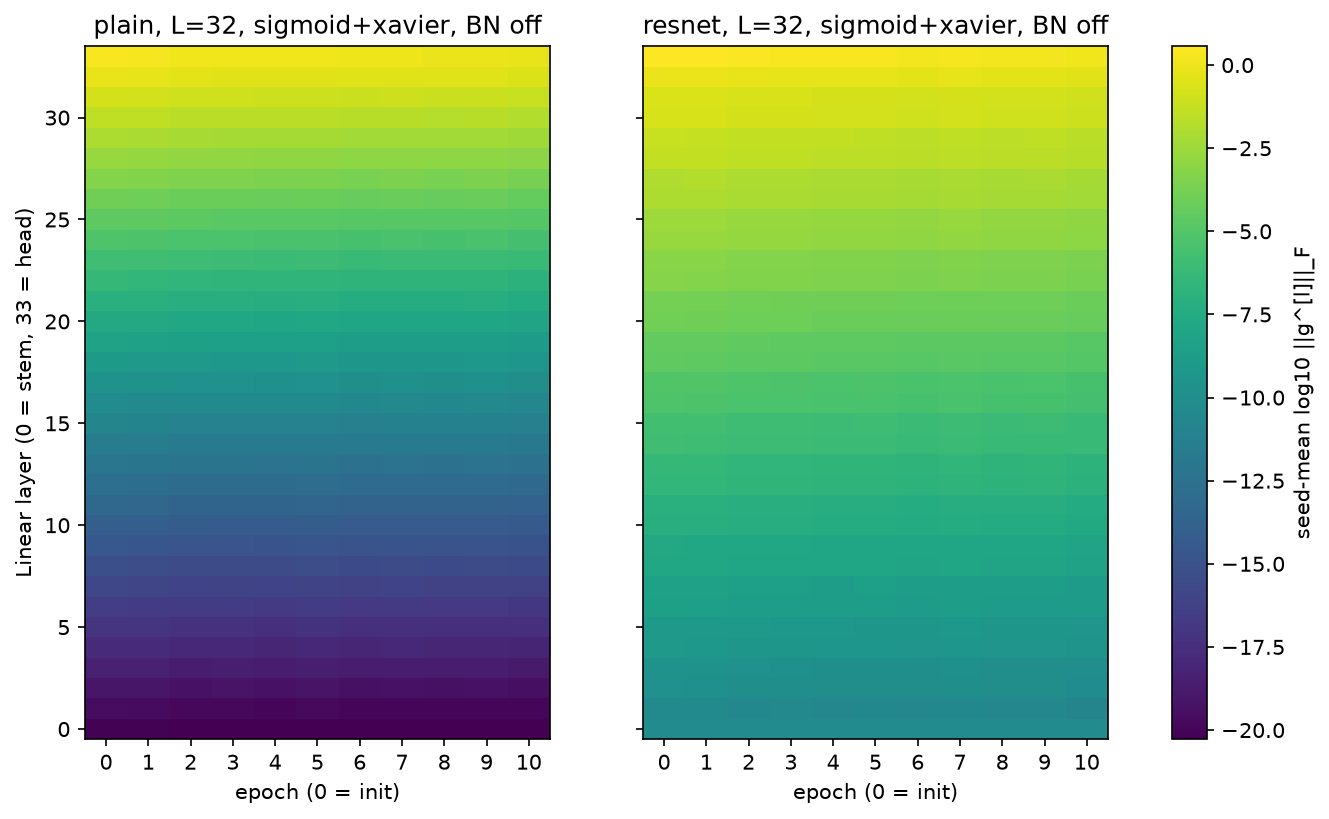
\includegraphics[width=\linewidth]{figures/heatmap_plain_vs_resnet.png}
\begin{figurecaptionmodern}
\capfig{Heatmap của $\log_{10}\left\|\mathbf{g}^{[l]}\right\|_F$ (trung bình trên
$3$ hạt giống, thang màu viridis chung cho hai panel, từ khoảng $-20$ đến $0$)
ở $L=32$, Sigmoid + Xavier, không BatchNorm. Trục hoành: epoch ($0$ = khởi tạo);
trục tung: chỉ số tầng tuyến tính ($0$ = stem, $33$ = head). Trái: PlainNet;
phải: ResNet. Kết luận: residual connection kéo stem từ khoảng $10^{-20.5}$
lên khoảng $10^{-10.8}$, nhưng gradient vẫn giảm theo hàm mũ từ head về stem
và không epoch nào thay đổi được điều đó.\label{fig:heatmap-plain-resnet}}
\end{figurecaptionmodern}
\end{figure}

\begin{figure}[htbp]
\centering
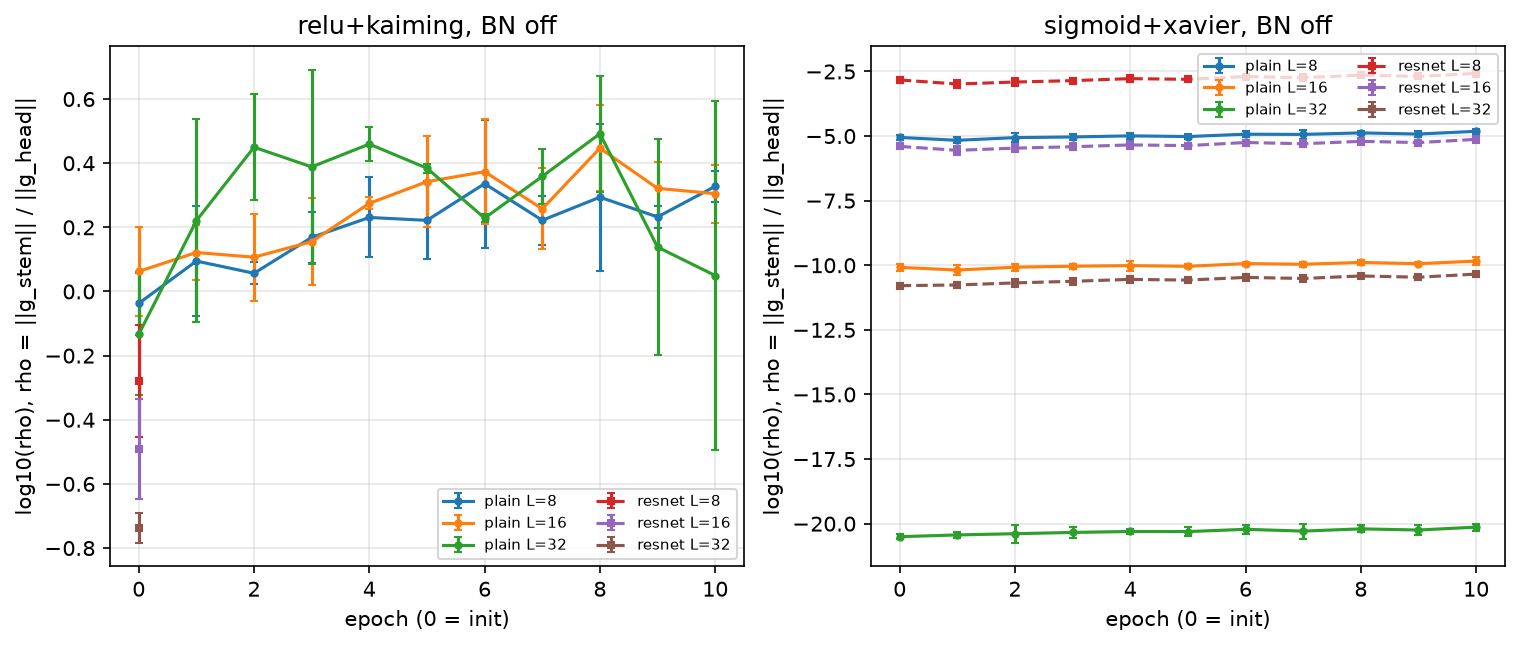
\includegraphics[width=\linewidth]{figures/gradient_flow_residual.png}
\begin{figurecaptionmodern}
\capfig{$\log_{10}\rho$ theo epoch ($0$ = khởi tạo), không BatchNorm; đường liền
là PlainNet, đường đứt là ResNet, mỗi màu một độ sâu $L\in\{8,16,32\}$, thanh
sai số là độ lệch chuẩn trên các hạt giống còn hữu hạn. Trái: ReLU + Kaiming;
phải: Sigmoid + Xavier. Kết luận: với sigmoid, mọi đường gần như nằm ngang suốt
$10$ epoch, nên huấn luyện không tự sửa được vanishing gradient; với ReLU,
ResNet không BN chỉ có điểm epoch $0$ vì mọi lần chạy đều phân kỳ ở epoch
$1$.\label{fig:gradflow-residual}}
\end{figurecaptionmodern}
\end{figure}

\paragraph{(a) Sigmoid ResNet với activation sau phép cộng vẫn vanishing.}
\emph{Cơ chế.} Đặt $\mathbf{s}_l = \mathbf{x}_l + F(\mathbf{x}_l)$. Jacobian
của một khối là
\[
  \frac{\partial\mathbf{x}_{l+1}}{\partial\mathbf{x}_l}
  \;=\; \operatorname{diag}\!\big(\sigma'(\mathbf{s}_l)\big)
        \left(\mathbf{I} + \frac{\partial F}{\partial\mathbf{x}_l}\right),
  \qquad \sigma'(\cdot)\le\tfrac14 .
\]
Identity path chỉ bảo vệ gradient \emph{bên trong} dấu ngoặc. Thừa số
$\operatorname{diag}(\sigma')$ nằm ngoài nên vẫn bị nhân một lần mỗi khối, và
chặn~\eqref{eq:governing} của Mục~\ref{sec:nguyennhan} vẫn áp dụng, chỉ với số
thừa số ít hơn. Trên đường ngắn nhất từ head về stem, PlainNet đi qua $L+1$
thừa số $\sigma'$ (stem cộng $L$ tầng ẩn), còn ResNet đi qua $L/2+1$ (stem cộng
$L/2$ activation sau phép cộng). Lý thuyết vì vậy dự báo
$\log_{10}\rho_{\text{ResNet}}/\log_{10}\rho_{\text{Plain}}\approx(L/2+1)/(L+1)$.

\emph{Bằng chứng.} Tại khởi tạo, $\log_{10}\rho$ của PlainNet là $-5.05$,
$-10.1$, $-20.5$ và của ResNet là $-2.83$, $-5.40$, $-10.8$ ở $L=8,16,32$. Tỉ
số đo được $0.560$, $0.536$, $0.526$ khớp với dự báo $5/9=0.556$,
$9/17=0.529$, $17/33=0.515$. Quy về mỗi thừa số $\sigma'$, hệ số suy giảm là
$0.23$--$0.27$, sát chặn $1/4$, ở cả hai kiến trúc.
Hình~\ref{fig:heatmap-plain-resnet} cho thấy trường gradient theo tầng không đổi
qua $10$ epoch, và Hình~\ref{fig:gradflow-residual} (phải) cho thấy
$\log_{10}\rho$ chỉ nhích $0.24$--$0.45$ sau $10$ epoch. Ở $L=32$, cập nhật
tương đối của stem ResNet chỉ còn $r/\epsilon_{32}\approx0.8\text{--}2.3\times10^{-8}$
(PlainNet: đúng $0$, mọi bước đều bị \texttt{torch.equal} xác nhận không đổi).
Độ chính xác test của cả $18$ lần chạy Sigmoid không BN ($6$ cấu hình) ở epoch $10$ đều là
$10.0\%$, tức mức đoán ngẫu nhiên.

\emph{Kết luận.} Residual connection chia đôi số mũ của vanishing gradient
nhưng không xoá nó; muốn identity path thực sự là đường cao tốc, activation
bão hoà phải nằm \emph{trong} nhánh $F$, không đặt sau phép cộng.

\paragraph{(b) ReLU ResNet không BatchNorm phân kỳ ngay epoch đầu.}
\emph{Cơ chế.} Không có BatchNorm, nhánh $F$ với khởi tạo Kaiming giữ phương sai
của đầu vào thay vì triệt tiêu nó, và phép cộng của identity path cộng dồn
phương sai qua từng khối:
\[
  \operatorname{Var}(\mathbf{x}_{l+1}) \;\approx\;
  \operatorname{Var}(\mathbf{x}_l) + \operatorname{Var}\big(F(\mathbf{x}_l)\big)
  \;=\; (1+\kappa)\operatorname{Var}(\mathbf{x}_l)
  \;\Longrightarrow\;
  \operatorname{Var}(\mathbf{x}_{L/2}) \approx (1+\kappa)^{L/2}\operatorname{Var}(\mathbf{x}_0),
\]
với $\kappa=\operatorname{Var}(F(\mathbf{x}_l))/\operatorname{Var}(\mathbf{x}_l)$
cỡ $1$. Phương sai của forward pass tăng theo hàm mũ của số khối, kéo theo
logits và gradient. PlainNet + Kaiming nhân phương sai với khoảng $1$ mỗi tầng
nên không cộng dồn.

\emph{Bằng chứng.} Phương sai forward không được đo trực tiếp, nhưng
$\mathbf{g}_{\text{head}} = \boldsymbol{\delta}_{\text{out}}\mathbf{a}^{\top}$ tỉ
lệ với độ lớn activation cuối. Tại khởi tạo, $\|\mathbf{g}_{\text{head}}\|_F$ của
ResNet là $51.8$, $313$, $1.26\times10^{4}$ ở $L=8,16,32$ ($4$, $8$, $16$ khối),
tức tăng khoảng $1.57$--$1.59$ lần mỗi khối về chuẩn, hay khoảng $2.5$ lần về
phương sai. PlainNet cùng cấu hình giữ ở $2.4$--$4.3$. Mất mát trên probe batch
lúc khởi tạo của ResNet là $9.90$, $41.8$, $1480$, so với $\ln 10\approx2.30$ của
một bộ phân loại ngẫu nhiên. Stem gnorm ở $L=32$ là $(2.32\pm0.244)\times10^{3}$
(Bảng~\ref{tab:training-dynamics}), nên bước SGD đầu tiên có
$\eta\|\mathbf{g}_{\text{stem}}\|_F\approx232$. Kết quả là $9/9$ lần chạy phân kỳ
ở epoch $1$, và mạng càng sâu thì càng sớm: bước $3$--$4$ ($L=8$), bước $2$
($L=16$), bước $1$ ($L=32$). Trong Hình~\ref{fig:gradflow-residual} (trái), các
đường ResNet chỉ còn điểm epoch $0$. PlainNet ReLU không BN cũng không hoàn toàn
an toàn: $1/3$ hạt giống ở $L=32$ phân kỳ (epoch $1$, bước $3$).

\emph{Kết luận.} Identity path chuyển phép \emph{nhân} của mạng thuần thành phép
\emph{cộng} của phương sai; không có cơ chế chuẩn hoá, phép cộng đó tự nó cộng
dồn thành bùng nổ.

\paragraph{(c) Ở $L=32$, BatchNorm + identity path giữ $\rho$ gần $1$ và
chuyển thành độ chính xác.}
\emph{Cơ chế.} BatchNorm ở cuối nhánh $F$ ép
$\operatorname{Var}(F(\mathbf{x}_l))\approx1$ bất kể $l$ (với $\gamma=1$,
$\beta=0$ lúc khởi tạo), nên phương trình ở (b) đổi từ nhân sang cộng:
\[
  \operatorname{Var}(\mathbf{x}_{l+1}) \approx \operatorname{Var}(\mathbf{x}_l) + 1
  \;\Longrightarrow\;
  \operatorname{Var}(\mathbf{x}_l) \approx \operatorname{Var}(\mathbf{x}_0) + l .
\]
Phương sai tăng tuyến tính chứ không theo hàm mũ, và tỉ trọng của nhánh $F$
so với identity path giảm cỡ $1/\sqrt{l}$. Vì vậy mỗi thừa số
$\mathbf{I}+\partial F/\partial\mathbf{x}_l$ gần $\mathbf{I}$, và tích của chúng
không trôi theo hàm mũ. PlainNet + BN không có identity path, nên gradient đi về
stem phải qua $L+1=33$ cặp BN--ReLU nối tiếp và không có gì giữ chúng gần
nhau.

\emph{Bằng chứng (Bảng~\ref{tab:training-dynamics}, phần trên).}
\begin{itemize}[leftmargin=*, itemsep=1pt]
  \item \textbf{$\rho$ của ResNet ở gần $1$.} Qua $11$ lần đo, $\log_{10}\rho$
    trung bình của ResNet nằm trong $[-0.914,\ 0.348]$, tức $\rho\in[0.122,\ 2.23]$.
    PlainNet bùng nổ về phía stem lúc khởi tạo ($\log_{10}\rho=2.81$,
    $\rho\approx643$, stem gnorm $626$), rồi rơi xuống $-1.30$ sau epoch $1$ và
    ở lại quanh $-1.2$ đến $-1.4$ ($\rho\approx0.05$).
  \item \textbf{Stem của ResNet được cập nhật mạnh hơn nhiều.} Ở epoch $10$,
    stem gnorm là $1.07\pm0.221$ (ResNet) so với $0.0469\pm0.0076$ (PlainNet),
    và cập nhật tương đối $r/\epsilon_{32}$ là $(5.08\pm0.46)\times10^{4}$ so với
    $423\pm76.4$, tức stem của ResNet học nhanh hơn khoảng $120$ lần.
  \item \textbf{Độ chính xác tương ứng.} Test acc ở epoch $10$ là
    $32.0\pm5.77\%$ (ResNet) so với $22.9\pm1.09\%$ (PlainNet). Theo từng hạt
    giống, ResNet đạt $38.5$, $29.9$, $27.5\%$ và PlainNet đạt $24.2$, $22.5$,
    $22.2\%$, nên mọi hạt giống ResNet đều vượt mọi hạt giống PlainNet.
\end{itemize}
Lợi thế này chỉ xuất hiện ở độ sâu lớn. Ở $L=8$ và $L=16$, PlainNet + BN nhỉnh
hơn ($35.1\pm4.10$ so với $31.6\pm5.72\%$; $29.5\pm2.88$ so với $28.2\pm6.75\%$).
Độ chính xác của PlainNet giảm đơn điệu theo $L$ ($35.1\to29.5\to22.9\%$), còn
ResNet gần như giữ nguyên ($31.6\to28.2\to32.0\%$).

\emph{Kết luận.} BatchNorm chặn sự cộng dồn phương sai, identity path giữ đường
gradient về stem; cần \emph{cả hai} thì stem mới học được ở $L=32$, và đó là
nguồn của khoảng cách $9$ điểm phần trăm.

\begin{notebox}
Số liệu chỉ có $3$ hạt giống và $10$ epoch trên $10{,}000$ ảnh, nên các khoảng
$\pm$ của ResNet ($4$--$7$ điểm phần trăm) còn rộng. Hai biến thể Sigmoid + BN
không được đưa vào Bảng~\ref{tab:training-dynamics}; ở $L=32$, chúng đạt
$18.9\pm3.55\%$ (PlainNet) và $22.3\pm6.47\%$ (ResNet) ở epoch $10$, với
$\log_{10}\rho$ trung bình của cả hai ở trong $[-0.41,\ 0.09]$ suốt quá trình huấn luyện.
BatchNorm một mình đã xoá vanishing gradient của sigmoid về mặt chuẩn gradient,
nhưng không đưa độ chính xác lên ngang ReLU + BN.
\end{notebox}

\section{Tổng kết và các nguyên lý khắc phục}
\label{sec:tongket}

Phần lớn lập luận của tài liệu xoay quanh một chặn trên, \eqref{eq:governing}:
\[
  \left\|\boldsymbol{\delta}^{[l]}\right\| \le c^{\,L-l}\left\|\boldsymbol{\delta}^{[L]}\right\|,
  \qquad
  c = \sigma_{\max}(\mathbf{W}) \cdot \max\sigma' .
\]
Chặn này chỉ nói một chiều: $c<1$ đủ để gradient co theo hàm mũ, còn $c\ge1$
không bảo đảm điều gì về giá trị thực (Mục~\ref{sec:thucnghiem} đo được
$c\approx2.4$--$2.68$ ở điều kiện ReLU + He mà không có bùng nổ). Các kỹ thuật
thực hành dưới đây có thể đọc như những cách nới hoặc tránh chặn đó --- một góc
nhìn hữu ích, không phải một định lý phân loại.

\begin{table}[H]
\centering
\renewcommand{\arraystretch}{1.25}\small
\begin{tabularx}{\linewidth}{@{}
  >{\raggedright\arraybackslash\hsize=0.80\hsize}X
  >{\raggedright\arraybackslash\hsize=1.15\hsize}X
  >{\raggedright\arraybackslash\hsize=0.85\hsize}X
  >{\raggedright\arraybackslash\hsize=1.20\hsize}X @{}}
\toprule
\rowcolor{rowLavender}
\textbf{Nguyên nhân} & \textbf{Biểu hiện toán học} &
\textbf{Kiến trúc bị ảnh hưởng} & \textbf{Nguyên lý khắc phục} \\
\midrule
Bão hoà hàm kích~hoạt &
$\max\sigma' = \tfrac14$ (sigmoid), $\to 0$ khi $|z|$ lớn &
MLP sâu, CNN đời đầu, RNN dùng $\tanh$ &
Thay bằng hàm không bão hoà: ReLU, LeakyReLU, GELU $\Rightarrow$ nâng
$\max\sigma'$ lên $1$ \\
\addlinespace[3pt]
Bán kính phổ lệch khỏi $1$ &
$\textstyle\prod_{k}\sigma_{\max}(\mathbf{W}^{[k]})$ phân kỳ hoặc tiêu biến &
Mọi mạng sâu; nhạy nhất ở mạng rất~sâu &
Khởi tạo có kiểm soát phương sai: Xavier, He $\Rightarrow$ đặt
$\sigma_{\max}(\mathbf{W})\approx1$ \\
\addlinespace[3pt]
Tiền kích hoạt trôi vào vùng bão~hoà &
$\mathbf{z}$ dịch xa $0$ theo chiều sâu, kéo $\sigma'\to0$ &
Mạng sâu huấn luyện lâu, dịch chuyển hiệp biến~nội &
Chuẩn hoá: BatchNorm, LayerNorm $\Rightarrow$ tái định tâm $\mathbf{z}$ quanh $0$ \\
\addlinespace[3pt]
Cấu trúc tích thuần tuý của Jacobian &
$\boldsymbol{\delta}^{[l]}$ là tích $L-l$ thừa số, không có số hạng bậc không &
Mạng rất sâu (trên $50$ tầng) &
Kết nối tắt: Jacobian thành $\mathbf{I}+\mathbf{F}'$ $\Rightarrow$ tích có
thêm số hạng $\mathbf{I}$ \\
\addlinespace[3pt]
Chia sẻ trọng số theo thời gian &
Chặn là $\sigma_{\max}(\mathbf{W}_{hh})^{T-1}$, không có trung bình hoá &
RNN thuần &
Cổng cộng tính: LSTM, GRU $\Rightarrow$ đường dẫn gần đồng nhất; cắt ngưỡng
gradient cho chiều bùng~nổ \\
\bottomrule
\end{tabularx}

\begin{captionbelowboxaivn}
Bảng 6: Phân loại nguyên nhân biến đổi gradient và nguyên lý khắc phục tương ứng,
đọc qua chặn trên $c = \sigma_{\max}(\mathbf{W})\cdot\max\sigma'$.
\end{captionbelowboxaivn}
\end{table}

\subsection{Bốn nguyên lý, đọc qua lăng kính của \texorpdfstring{$c$}{c}}

\textbf{ReLU và GELU --- nâng $\max\sigma'$.} Với $\mathrm{ReLU}(z)=\max(0,z)$,
đạo hàm bằng $1$ trên toàn miền dương thay vì bị chặn bởi $1/4$. Thừa số
$\max\sigma'$ trong $c$ nhảy từ $0.25$ lên $1$, tức chặn trên không còn ép
gradient co bốn lần mỗi tầng; hệ số thực còn tuỳ tỉ lệ nơ-ron hoạt động. Giá phải trả là nơ-ron chết ($\sigma'=0$ vĩnh viễn trên nhánh
âm), điều mà LeakyReLU và GELU khắc phục bằng cách giữ một độ dốc nhỏ khác không.
Trong thực nghiệm ở Mục~\ref{sec:thucnghiem} (cùng với khởi tạo He), cặp này
giữ $\log_{10}\rho$ trong khoảng $-0.74$ đến $-0.53$ ở $L\le20$, so với
$-12.7$ của sigmoid + Xavier ở $L=20$ --- đó là kết quả tại bước khởi tạo, trên
một kiến trúc cụ thể, không phải một đảm bảo chung.

\textbf{Xavier và He --- điều khiển $\sigma_{\max}(\mathbf{W})$.} Hai sơ đồ khởi
tạo chọn phương sai trọng số sao cho phương sai tín hiệu được bảo toàn khi đi qua
tầng. Chúng điều khiển độ lợi \emph{trung bình bình phương}, không phải
$\sigma_{\max}(\mathbf{W})$: với ma trận $64\times64$, thực nghiệm đo được
$\sigma_{\max}\approx1.8$--$1.9$ (Xavier) và chặn $c\approx2.4$--$2.68$ (He), tức chặn
trên $c$ không về $1$ dù gradient thực không bùng nổ. Xavier~\cite{GlorotBengio2010} dung hoà ràng buộc tiến và ngược bằng
$\operatorname{Var}(w)=2/(n_{\text{in}}+n_{\text{out}})$; He~\cite{He2015} dùng
$\operatorname{Var}(w)=2/n_{\text{in}}$, với hệ số $2$ bù cho việc ReLU triệt tiêu
một nửa số nơ-ron. Đây là một trong những can thiệp rẻ nhất: nó không tốn thêm phép tính nào
sau bước khởi tạo.

\textbf{BatchNorm và LayerNorm --- giữ $\mathbf{z}$ ngoài vùng bão hoà.} Khởi tạo
chỉ tác động lên phân phối tiền kích hoạt ở bước $0$; khi huấn luyện tiến triển, phân phối của
$\mathbf{z}$ trôi đi và có thể trượt vào vùng bão hoà, kéo $\max\sigma'$ xuống.
Chuẩn hoá~\cite{IoffeSzegedy2015} tái định tâm và tái co giãn $\mathbf{z}$ ở mỗi
bước, giữ nó quanh gốc nơi $\sigma'$ đạt cực đại. Nói cách khác, chuẩn hoá
giúp \emph{duy trì} trong quá trình huấn luyện điều kiện mà khởi tạo chỉ đặt
ở bước đầu --- trong phạm vi các giả thiết của nó (lô đủ lớn với BatchNorm,
tham số co giãn học được không trôi quá xa).

\textbf{Kết nối tắt --- phá vỡ cấu trúc tích.} Ba biện pháp trên đều cố đưa $c$
về $1$, nhưng vẫn chấp nhận rằng gradient là một \emph{tích}. ResNet~\cite{He2016ResNet}
tấn công chính cấu trúc đó. Với khối $\mathbf{a}^{[l]} = \mathbf{a}^{[l-1]} +
\mathcal{F}(\mathbf{a}^{[l-1]})$, Jacobian giữa hai tầng trở thành
\[
  \frac{\partial\mathbf{a}^{[l]}}{\partial\mathbf{a}^{[l-1]}}
  = \mathbf{I} + \mathcal{F}'(\mathbf{a}^{[l-1]}).
\]
Tích của các ma trận dạng $\mathbf{I}+\mathcal{F}'$ khai triển thành
$\mathbf{I} + \sum_k \mathcal{F}'_k + (\text{các số hạng bậc cao})$: luôn có
một số hạng \emph{bậc không} bằng đúng $\mathbf{I}$. Số hạng này không suy giảm
theo chiều sâu; tổng vẫn có thể nhỏ hơn nếu các số hạng khác triệt tiêu một
phần với nó, nhưng khi các nhánh $\mathcal{F}'_k$ nhỏ lúc khởi tạo thì đường tắt
chiếm ưu thế. Đây là một lý do quan trọng khiến He và cộng sự huấn luyện được
mạng $152$ tầng, trong khi trong cùng bài báo, mạng thuần tích $34$ tầng có sai
số huấn luyện \emph{cao hơn} mạng thuần tích $18$ tầng. Về mặt nguyên lý, đây
đúng là cơ chế mà cổng LSTM dùng trong miền thời gian (Mục~\ref{sec:bptt}), chỉ
chuyển sang miền chiều sâu.

\begin{guidelinebox}{Thứ tự ưu tiên khi gặp mạng sâu không học được}
$(1)$ Xác nhận đây là vấn đề tối ưu hoá bằng cách kiểm tra sai số \emph{huấn
luyện}. $(2)$ In bảng chuẩn gradient theo tầng. $(3)$ Nếu triệt tiêu: đổi sang
ReLU/GELU và khởi tạo He --- đây là hai thay đổi rẻ nhất, thường đủ. $(4)$ Nếu
vẫn chưa đủ: thêm chuẩn hoá. $(5)$ Nếu mạng rất sâu: thêm kết nối tắt. $(6)$ Nếu
bùng nổ: cắt ngưỡng gradient trước, rồi mới xem lại khởi tạo.
\end{guidelinebox}

\subsection{Liên hệ với tài liệu Module 4}

Các chủ đề trên được phát triển đầy đủ, kèm chứng minh chi tiết và mã nguồn đã
thực thi, trong sổ tay \texttt{docs/module4-deeplearning-optimization.tex}:

\begin{itemize}[leftmargin=*, itemsep=2pt]
  \item \textbf{Mục 11} --- Hàm kích hoạt và đạo hàm: họ bão hoà so với họ không
    bão hoà, softmax và cross-entropy.
  \item \textbf{Mục 13} --- Triệt tiêu, bùng nổ gradient và khởi tạo trọng số:
    chứng minh đầy đủ định lý Xavier/Glorot và He/Kaiming.
  \item \textbf{Mục 14} --- Điều hoà và chuẩn hoá: inverted dropout,
    BatchNorm, so sánh các sơ đồ chuẩn hoá.
  \item \textbf{Mục 18} --- Kết nối tắt và dòng chảy gradient: phân tích khai
    triển $\mathbf{I}+\mathcal{F}'$ và ý nghĩa với mặt mất mát.
\end{itemize}

Tài liệu hiện tại đóng vai trò dẫn nhập tập trung vào \emph{nguyên nhân}; sổ tay
Module 4 bao quát toàn bộ không gian giải pháp và lý thuyết tối ưu hoá đi kèm.


\printbibliography[title={Tài liệu tham khảo}]

\end{document}
